\documentclass{config/apuntes}

\title{Análisis de Imagen Biomédica}
\author{Sandra Mingo Ramírez}
\date{2025/26}
\acronym{AIBM}

\usepackage[all]{nowidow}
\usepackage{listing}
\usepackage{color}
\usepackage{tabularx}
\usepackage{multirow}
\usepackage{makecell}
\usepackage{amsmath}
\usepackage{array}
\usepackage{soul}

\definecolor{dkgreen}{rgb}{0,0.6,0}
\definecolor{gray}{rgb}{0.5,0.5,0.5}
\definecolor{mauve}{rgb}{0.58,0,0.82}

\lstset{
  frame=tb,
  aboveskip=3mm,
  belowskip=3mm,
  showstringspaces=false,
  columns=flexible,
  basicstyle={\small\ttfamily},
  numbers=none,
  numberstyle=\tiny\color{gray},
  keywordstyle=\color{blue},
  commentstyle=\color{dkgreen},
  stringstyle=\color{mauve},
  breaklines=true,
  breakatwhitespace=true,
  tabsize=3
}

\usepackage{tocloft}

\advance\cftchapnumwidth 0.9em\relax
\advance\cftsecnumwidth 0.6em\relax
\advance\cftsubsecindent 0.5em\relax
\advance\cftsubsecnumwidth 0.5em\relax
\begin{document}

\begin{abstract}
En las ciencias biomédicas no solo se recogen datos; en ocasiones se generan imágenes que posteriormente se deben analizar y de las que se debe extraer información comprensiva. 
El análisis de imagen biomédica es el proceso de examinar y extraer información útil de imágenes biomédicas, como resonancias magnéticas, tomografías computarizadas (TC) o ecografías, para facilitar diagnósticos, monitorear el progreso de enfermedades y desarrollar nuevas técnicas de diagnóstico y tratamiento. El prefijo "bio" se refiere a la fase preclínica, siendo así las imágenes de modelos animales fundamentalmente.
\end{abstract}

\pagestyle{plain}

\maketitle

\tableofcontents

%2 profesores y 2 invitados
%3 aplicaciones: microscopía, PET y resonancia magnética
% 60 % examen -> convocatoria en enero,
% 15 % Moodle
% 25 % pequeños trabajos

% Programación en Matlab - versión gratuita para estudiantes, 
% Octave alternativa gratuita a Matlab

%16/09 - Blanca Lizarbe
\chapter{Introducción al procesado de imágenes}
\section{Formación de imágenes}
Hay muchas formas de obtener una imagen, dependiendo de la fuente de energía (p. ej., fotones, ondas de radio, ultrasonido) y del sistema detector que la capture. Los tipos de imágenes se clasifican según si la formación es directa o indirecta, analógica (continua) o digital, y según el tipo de energía utilizada (radiación electromagnética, acústica, etc.).

Una forma de clasificarlas es en función del tipo de energía o radiación utilizada. La luz visible es una pequeña parte del espectro electromagnético. Las imágenes biomédicas pueden generarse utilizando otras partes de este espectro (rayos X, radiofrecuencia), así como otras formas de energía como ondas mecánicas (sonar, ultrasonido) o campos (magnéticos, eléctricos).

Aunque el grueso del curso sea el análisis y procesado de las imágenes, es importante saber de dónde vienen y su contexto.
\begin{itemize}
\item La \textbf{formación de imagen de rayos X} proviene de una fuente emisora. Estos rayos interaccionan con el tejido biológico (son atenuados principalmente por absorción y dispersión). La radiación que atraviesa el tejido incide sobre un detector (que históricamente era una placa fotográfica o de película, pero hoy son casi exclusivamente detectores digitales como placas de fósforo o detectores planos).
\item La \textbf{formación de una imagen de Resonancia Magnética (RM)} se basa en aplicar un campo magnético estático y fuerte (B0) al tejido, alineando los momentos magnéticos de los núcleos de hidrógeno. Se aplican pulsos de radiofrecuencia (RF) para excitar estos núcleos, que al relajarse emiten señales de RF. Esta señal se detecta con bobinas. Utilizando gradientes de campo magnético (que varían el campo de forma lineal en el espacio), se puede codificar espacialmente la señal y reconstruirla digitalmente para asignar diferentes intensidades de señal a cada voxel (elemento de volumen 3D) o píxel (2D).
\end{itemize}

\subsection{De analógico a digital}
Para convertir una imagen analógica (como una placa de rayos X o una fotografía) a digital se utiliza un dispositivo de digitalización, como un escáner o un detector digital directamente. Este proceso implica \textbf{muestrear (sampling)} la imagen, dividiendo el espacio en una matriz discreta de elementos (píxeles), y \textbf{cuantizar} la intensidad de luz en cada punto, asignándole un valor digital discreto.

La resolución espacial tiene que ver con el nivel de detalle discernible, determinado por el tamaño del píxel y las propiedades del sistema de imagen. Una imagen con muchos píxeles pequeños (alta resolución) permite visualizar detalles finos y bordes definidos. En cambio, una imagen de baja resolución tiene pocos píxeles grandes, lo que resulta en una pérdida de detalles y una apariencia pixelada o borrosa al ampliarla.

Las imágenes con las que se suele trabajar en diagnóstico por imagen suelen representarse en escala de grises. Esto significa que a cada píxel se le asigna una intensidad lumínica representada por un valor numérico. En el formato estándar de 8 bits, este valor va de 0 (negro) a 255 (blanco), permitiendo $2^8 = 256$ tonos de gris intermedios. La cantidad de bits utilizada para representar el valor de un píxel se denomina profundidad de bits (bit depth).
%Importante el concepto de 256 niveles de gris y los 8 bits

Cualquier sistema moderno de formación de imagen biomédica integra \textbf{sensores} (o detectores) y un \textbf{conversor de analógico a digital (ADC).} La imagen digital se debe guardar, procesar y, en ocasiones, se reconvierte a analógico (por ejemplo, mediante una pantalla) para su visualización.

\section{Procesado de imágenes digitales}
Dentro del procesamiento de imagen hay varias categorías o pasos:
\begin{enumerate}
\item \textbf{Mejora o Realce de la Imagen (Image Enhancement):} Técnicas para ajustar propiedades como el brillo, el contraste o para aplicar filtros (como la convolución) con el fin de hacer ciertas características más visibles para el observador humano o para un algoritmo posterior. Incluye la corrección de algunos artefactos.
\item \textbf{Restauración de Imagen (Image Restoration):} Su objetivo es eliminar o reducir la degradación (como el desenfoque o el ruido) utilizando un modelo de cómo se degradó la imagen. Se busca aproximarse a la imagen original no degradada.
\item \textbf{Análisis de la Imagen (Image Analysis):} Procesos como la segmentación (delimitación de regiones de interés), la extracción de características (cálculo de métricas cuantitativas) y la clasificación de objetos.
\item \textbf{Compresión de Imagen (Image Compression):} Técnicas para reducir el tamaño de los archivos de imagen para su almacenamiento o transmisión eficiente (p. ej., JPEG, JPEG 2000, DICOM con compresión).
\item \textbf{Síntesis de Imagen (Image Synthesis):} Generación de imágenes a partir de modelos o datos, como en la reconstrucción tomográfica o la generación de imágenes mediante Inteligencia Artificial.
\end{enumerate}

\subsection{Image enhancement}
Las imágenes biomédicas se utilizan para el diagnóstico, tanto \textbf{cualitativo} (observación visual de morfología) como \textbf{cuantitativo} (medición de parámetros fisiológicos o bioquímicos). Para el diagnóstico cualitativo, se tratan las imágenes para reducir ruido o realzar bordes. En las imágenes cuantitativas, el valor numérico del píxel tiene significado físico (p. ej., unidades Hounsfield en TC, concentración de un contraste, valores T1 o T2 en RM). Por ello, al manipular estas imágenes para su análisis, es crucial utilizar técnicas que no alteren o que corrijan de manera controlada los valores subyacentes, preservando la información biológico-física. A menudo, la consistencia en el procesamiento (aplicar el mismo algoritmo a todos los sujetos de un estudio) es más importante que la absolutez del valor.

Los \textbf{artefactos} son patrones o estructuras presentes en la imagen que no corresponden a la anatomía o fisiología real del sujeto, sino que son causados por el equipo, el protocolo de adquisición o el propio paciente. Estos incluyen desde artefactos por metal (implantes) hasta los causados por el movimiento voluntario o involuntario del paciente durante una adquisición, especialmente si es larga. La \textbf{reducción de ruido} (ruido aleatorio inherente a cualquier medición física) es también esencial para mejorar la relación señal-ruido (SNR).

Hoy día, las técnicas de \textbf{aprendizaje automático (machine learning),} y en particular las \textbf{redes neuronales convolucionales (CNN),} se utilizan extensamente. Un ejemplo es el entrenamiento de redes con pares de imágenes: una entrada degradada (p. ej., con artefactos de movimiento o ruido) y una salida objetivo de referencia ("ground truth") de alta calidad. La red aprende la transformación para mapear la imagen defectuosa a una versión corregida. Es importante destacar que a menudo el "ground truth" perfecto no existe \textit{in vivo}, por lo que los modelos se entrenan con datos simulados o con imágenes de alta calidad adquiridas en condiciones ideales.

Para corregir el ruido, una técnica común es el \textbf{filtrado espacial}. Un ejemplo básico es el \textbf{filtro Gaussiano}, que suaviza la imagen promediando los valores de los píxeles vecinos, ponderados por una función Gaussiana. Esto homogeniza las regiones y reduce el ruido, pero a costa de una potencial pérdida de detalle (suavizado de bordes). La operación se aplica deslizando un kernel (ventana) sobre la imagen, realizando una \textbf{convolución} (producto punto entre el kernel y los píxeles subyacentes) en cada posición.

\begin{figure}[h]
\centering
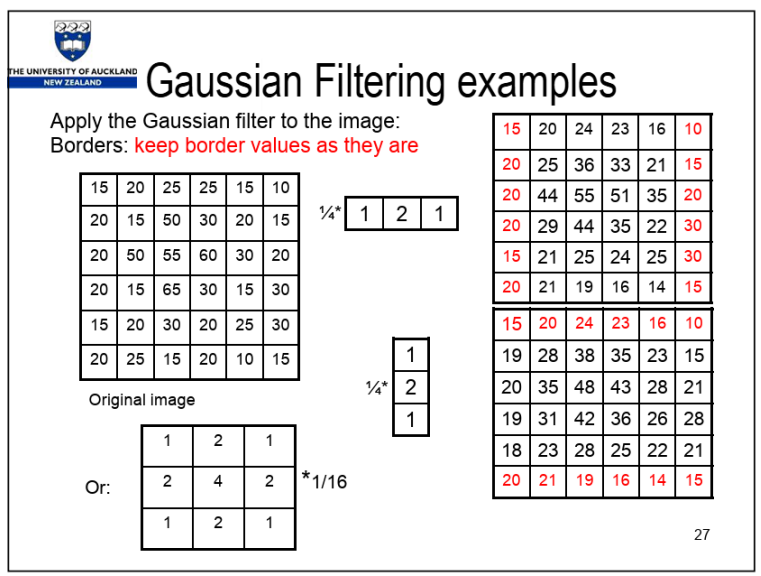
\includegraphics[width = 0.8\textwidth]{figs/gaussian-filter.png}
\caption{Ejemplo de filtro Gaussiano. Se aplica la matriz izquierda inferior sobre la imagen original, multiplicando los valores por la matriz de filtro y dividiendo por 16. Esto se realiza sobre cada píxel a excepción de los bordes. Por ejemplo, para el píxel con valor 15 de la segunda fila, segunda columna: $(15*1 + 20 * 2 + 25 * 1 + 20 * 2 + 15 * 4 + 50 * 2 + 20 * 1 + 50 * 2 + 55 * 1)/16 = 455/16 = 28,4375 \approx 28$, que es el valor del píxel de la matriz derecha inferior.}
\end{figure}

Mejora de la Resolución: El término general es superresolución (super-resolution). Este proceso busca estimar o reconstruir una imagen de alta resolución a partir de una o varias imágenes de baja resolución. El objetivo es recuperar detalles finos perdidos durante la adquisición, lo que conduce a una visualización más clara y puede facilitar un diagnóstico más preciso. Es importante distinguirlo de un simple zoom o interpolación, que agranda los píxeles sin añadir información nueva real. Las técnicas de superresolución pueden ser:
\begin{itemize}
\item \textbf{Basadas en reconstrucción:} Utilizan múltiples imágenes sub-píxel de la misma escena y algoritmos para fusionarlas.
\item \textbf{Basadas en aprendizaje:} Utilizan redes neuronales (como CNNs) entrenadas con pares de imágenes (baja/alta resolución) para aprender el mapeo que añade los detalles faltantes.
\end{itemize}

\subsection{Image analysis}
La \textbf{segmentación} es un paso fundamental en el análisis de imágenes. Su objetivo es dividir una imagen en regiones o estructuras significativas, permitiendo extraer y cuantificar la información de interés. Por ejemplo, aislar solo los huesos en una Tomografía Computarizada (TC), delimitar un tumor, o separar el ventrículo izquierdo en una imagen cardiaca.

Se lleva a cabo mediante algoritmos que identifican boundaries (bordes) o regiones homogéneas basándose en propiedades como la intensidad, el color, la textura o el contexto. No se limita solo a la extracción de bordes; existen múltiples enfoques:
\begin{itemize}
\item Basados en umbral (thresholding): Separan según el valor de intensidad.
\item Basados en regiones (region growing, watershed): Agrupan píxeles conectados con propiedades similares.
\item Basados en bordes (edge detection): Identifican discontinuidades en la intensidad (usando operadores como Sobel, Canny).
\item Basados en modelos (active contours, level sets): Utilizan curvas o superficies que evolucionan para ajustarse a los contornos.
\item Basados en aprendizaje (Machine/Deep Learning): Las redes neuronales (especialmente las U-Net) aprenden a segmentar a partir de ejemplos etiquetados.
\end{itemize}

El \textbf{registro de imágenes (Image Registration)} es el proceso de alinear geométricamente dos o más conjuntos de imágenes (datasets) adquiridas en diferentes momentos, desde diferentes modalidades o desde distintos puntos de vista. El objetivo es establecer una correspondencia punto a punto entre ellas para poder comparar, fusionar o analizar la información de forma coherente.

Esto se logra encontrando la transformación espacial óptima que mapea los puntos de una imagen (imagen móvil o "moving") sobre los de otra (imagen de referencia o "fixed"). Los tipos de transformación, ordenados de menor a mayor complejidad y flexibilidad, son:
\begin{itemize}
\item \textbf{Registro rígido (Rigid):} Alinea imágenes solo con rotaciones y traslaciones (desplazamientos) globales. Preserva las distancias y ángulos entre todos los puntos. Es útil para imágenes de la misma anatomía sin cambios internos (p. ej., cabeza en diferentes estudios de RM).
\item \textbf{Registro por similitud (Similarity):} Añade escalado isotrópico (mismo factor de escala en todos los ejes) a la transformación rígida. Preserva las formas y los ángulos, pero no las distancias absolutas.
\item \textbf{Registro afín (Affine):} Incluye cizallamiento (shearing) y escalado anisotrópico (diferente factor en cada eje), además de las transformaciones rígidas y de escalado. Las líneas paralelas siguen siéndolo después de la transformación, pero los ángulos pueden no conservarse. Es útil para corregir diferencias de adquisición o geometría entre modalidades.
\item \textbf{Registro no rígido o deformable (Non-rigid/Deformable):} Maneja deformaciones elásticas o fluidas complejas, localizadas y no lineales. Es esencial para compensar movimientos de órganos (como el corazón o los pulmones), cambios anatómicos (crecimiento de un tumor) o para alinear imágenes de pacientes diferentes en un atlas poblacional.
\end{itemize}

%17/09 - Álvaro García
\chapter{Fundamentos imagen biomédica}
\section{Percepción visual}
\subsection{Fenómeno de la luz}
Una fuente de luz \textbf{monocromática} emite radiación predominantemente en una única \textbf{longitud de onda} (o frecuencia), percibida como un color puro. Un ejemplo característico es el láser. Por el contrario, la luz \textbf{policromática} está compuesta por una mezcla de múltiples longitudes de onda, como la luz solar o la de una bombilla LED blanca.

Existen dos tipos de fuentes luminosas:
\begin{itemize}
\item \textbf{Fuentes Primarias o Emisivas:} Generan su propia luz mediante procesos de excitación de átomos o moléculas (ej.: el Sol, una bombilla, un LED).
\item \textbf{Fuentes Secundarias o Reflectantes:} No generan luz propia, sino que reflejan total o parcialmente la luz que reciben de una fuente primaria (ej.: la Luna, un libro, la mayoría de los objetos que nos rodean). Casi todo lo que vemos son fuentes secundarias.
\end{itemize}

\subsection{Sistema visual humano}
El proceso de la visión comienza cuando la luz entra en el ojo y es proyectada sobre la \textbf{retina}, donde los \textbf{fotorreceptores} la captan y la convierten en señales electroquímicas (proceso de \textbf{transducción}). Estas señales se transmiten a través del \textbf{nervio óptico} al cerebro, donde se interpretan para generar la percepción visual.

Desde un punto de vista óptico, el ojo humano es análogo a una cámara fotográfica:
\begin{itemize}
\item \textbf{Lente:} El cristalino (junto con la córnea y los humores acuoso y vítreo) se encarga de enfocar la luz, proyectando una imagen nítida sobre la retina. Su forma se ajusta en un proceso llamado acomodación.
\item \textbf{Diafragma}: El iris (la parte coloreada) actúa como un diafragma, controlando el tamaño de la pupila para regular la cantidad de luz que entra en el ojo.
\item \textbf{Sensor}: La retina equivale al sensor de una cámara (CCD/CMOS). Es una capa de tejido sensible a la luz ubicada en la parte posterior del ojo.
\end{itemize}

La retina contiene dos tipos principales de fotorreceptores:
\begin{itemize}
\item \textbf{Bastones}: Altamente sensibles a la intensidad lumínica (luminancia), pero no al color. Son responsables de la visión escotópica (visión en condiciones de baja iluminación). Se concentran en la periferia de la retina, siendo muy sensibles al movimiento.
\item \textbf{Conos}: Menos sensibles que los bastones, pero especializados en la percepción del color (visión fotópica, en condiciones de alta iluminación). Se concentran en la fóvea, la zona central de la retina de máxima agudeza visual. Existen tres tipos, cada uno con un pico de sensibilidad a diferentes longitudes de onda: rojo (larga), verde (media) y azul (corta).
\end{itemize}

La capacidad del ojo tiene limitaciones físicas. La \textbf{resolución espacial} (capacidad para discernir detalles finos) y la \textbf{resolución temporal} (capacidad para discernir eventos rápidos) son finitas debido al número limitado de fotorreceptores y a su tiempo de respuesta.

La \textbf{agudeza visual} es la capacidad de distinguir entre dos puntos separados. Si la separación angular entre ellos es superior a \textbf{1 minuto de arco} (1/60 de grado), estimulan fotorreceptores y fibras nerviosas diferentes, por lo que el cerebro los percibe como entidades distintas. Si la separación es menor, ambos puntos estimulan el mismo receptor, y el cerebro percibe una \textbf{mezcla aditiva espacial (MAE)}, fusionándolos en un solo estímulo de color.

\begin{figure}[h]
\centering
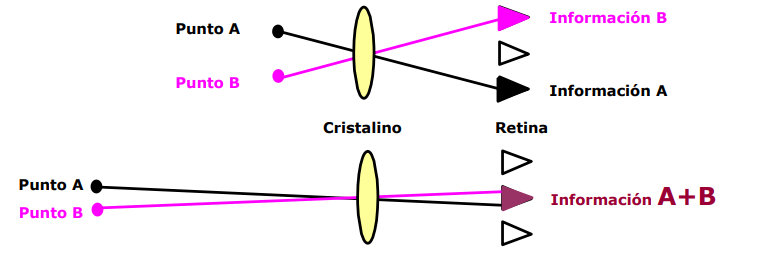
\includegraphics[width = \textwidth]{figs/mae.png}
\caption{Ilustración del principio de la mezcla aditiva espacial. Puntos de color suficientemente pequeños y cercanos se perciben como un color uniforme.}
\end{figure}

Este principio es fundamental en tecnologías de visualización como las pantallas de televisión y monitores, donde la imagen se forma mediante \textbf{píxeles} compuestos por subpíxeles rojos, verdes y azules (triadas de colores) cuya separación es inferior al umbral de agudeza visual.

La \textbf{memoria visual} o persistencia retiniana es una propiedad por la cual la excitación de los fotorreceptores no cesa instantáneamente tras desaparecer el estímulo, sino que continúa enviando señales al cerebro durante un breve periodo. La integración de impulsos luminosos consecutivos da lugar a la sensación de continuidad, un fenómeno conocido como \textbf{mezcla aditiva temporal (MAT)} o persistencia retiniana.

\begin{figure}[h]
\centering
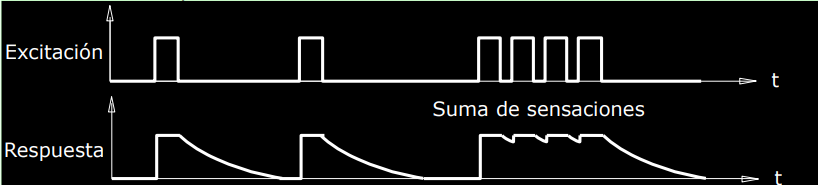
\includegraphics[width = \textwidth]{figs/mat.png}
\caption{Ilustración del principio de la mezcla aditiva temporal. Estímulos discretos sucesivos se perciben como un continuo si la frecuencia es suficientemente alta.}
\end{figure}

Si el intervalo entre impulsos es mayor de aproximadamente 40-50 ms (equivalente a 20-25 Hz), se percibe un parpadeo o \textit{flicker} molesto. Por debajo de este umbral, la respuesta al nuevo estímulo se suma a la anterior, creando una sensación de flujo continuo. Esto explica por qué una secuencia de imágenes estáticas (fotogramas) a una velocidad superior a 25 fps (fotogramas por segundo) se percibe como movimiento continuo. El umbral exacto varía con la luminancia y el campo visual estimulado.

\subsection{Luz}
La visión de los objetos no emisivos se debe a la reflexión (y en algunos casos, a la transmisión) de la luz que incide sobre ellos. La intensidad de la luz reflejada ($L$, luminancia) que llega al ojo depende de la intensidad de la luz incidente ($E$, iluminancia, medida en lux) y de las propiedades reflectivas del material ($R$).

En términos generales, se puede modelar como:
$$C_R(X, V, geom, t, \lambda) = E(X, t, \lambda).r(V, geom, \lambda)$$

Donde:
$R(V, \text{geom}, \lambda)$ es la reflectancia del material, que depende del ángulo de visión ($V$), la geometría de la superficie (si es rugosa/difusa o lisa/especular) y la longitud de onda ($\lambda$). Un objeto parece de un color porque absorbe selectivamente ciertas longitudes de onda y refleja otras.

Existen dos modelos de síntesis de color:
\begin{itemize}
\item \textbf{Síntesis Aditiva}: Propia de las fuentes de luz primarias. Los colores se crean sumando diferentes longitudes de onda de luz. La suma de los colores primarios aditivos (Rojo, Verde, Azul - RGB) en su máxima intensidad produce la percepción de blanco. Ej.: pantallas, monitores.
\item \textbf{Síntesis Sustractiva}: Propia de los pigmentos y materiales (fuentes secundarias). Los colores se crean porque el material absorbe (sustrae) ciertas longitudes de onda de la luz blanca incidente y refleja otras. Los colores primarios sustractivos son Cian, Magenta y Amarillo (CMY). La "suma" teórica de los tres absorbería toda la luz, produciendo negro. Ej.: pintura, impresión.
\end{itemize}

\subsection{Percepción de luminancia y color}
El sistema visual humano opera en tres regímenes de visión según el nivel de iluminación:
\begin{itemize}
\item \textbf{Visión Escotópica}: Activada en condiciones de muy baja iluminación (noche). Dominada por los bastones. No permite la percepción del color (visión en escala de grises) y tiene una baja agudeza visual.
\item \textbf{Visión Fotópica}: Activada en condiciones de alta iluminación (día). Dominada por los conos. Permite la percepción del color y una alta agudeza visual.
\item \textbf{Visión Mesópica}: Régimen intermedio (amanecer, atardecer, iluminación tenue). Participan tanto bastones como conos. La percepción del color y la agudeza visual son intermedias.
Los colores y nuestros conos no son puros. Los conos verdes absorben más que los conos rojos y azules. Nuestro cerebro recibe la información de los tres sensores y los integra para percibir un color u otro. 
\end{itemize}

La respuesta espectral de los tres tipos de conos se solapa. El cerebro deduce el color percibido (\textbf{crominancia}) a partir de la \textbf{señal tricromática} comparada que envían estos tres tipos de receptores. La crominancia se describe mediante dos atributos:
\begin{itemize}
\item \textbf{Tono:} el color en sí mismo.
\item \textbf{Saturación:} la pureza o intensidad del color.
\end{itemize}

Por otro lado, la \textbf{luminancia} se refiere a la cantidad de luz medida físicamente (en candelas/$m^2$), que se percibe subjetivamente como \textbf{brillo} en una escala de grises.


\begin{figure}[h]
\centering
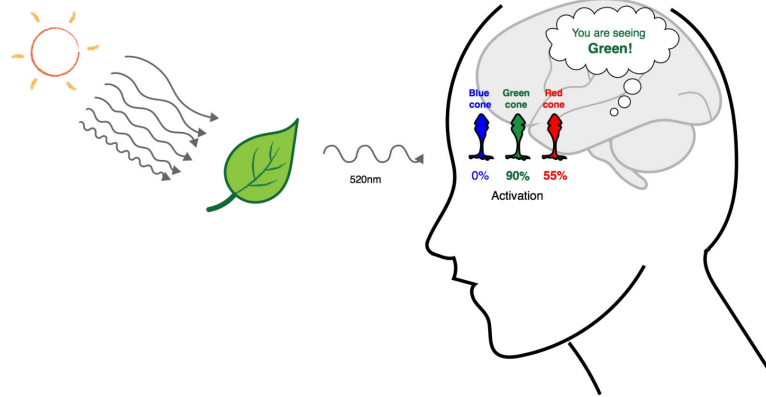
\includegraphics[width = \textwidth]{figs/perception.png}
\caption{Representación de la percepción visual, desglosando la información en componentes de luminancia (brillo) y crominancia (tono y saturación).}
\end{figure}

\subsection{Brillo}
El brillo es la percepción subjetiva de la luminancia. El sistema visual es extraordinariamente adaptable, capaz de funcionar en un rango de aproximadamente $10^{10}$ niveles de intensidad lumínica mediante el proceso de adaptación (ajuste de la sensibilidad retinal según la luminancia media del entorno).

La percepción del brillo es relativa, no absoluta. Depende críticamente del contraste entre un objeto y su fondo o entorno inmediato (Ley de Weber-Fechner). El ojo es mucho más sensible a las variaciones de luminancia (bordes, movimientos) que a los valores constantes.

No existe una medida física directa del brillo, ya que es una experiencia perceptiva compleja. En condiciones de alta luminancia (visión fotópica), el ojo tiene una mayor agudeza para discernir objetos claros sobre fondos oscuros. En condiciones de baja luminancia (visión escotópica o mesópica), la sensibilidad cambia, y puede resultar más fácil discernir objetos de luminancia media. 

Dado que la percepción del brillo es relativa, su evaluación debe considerar necesariamente el entorno. La \textbf{evaluación del contraste} es, por tanto, la medición cuantitativa de la diferencia percibida en luminancia (brillo) entre un objeto de interés (por ejemplo, un texto) y su fondo inmediato. Esta diferencia se expresa comúnmente como una razón de contraste (por ejemplo, 4:1, 7:1), que se calcula dividiendo la luminancia relativa de la parte más clara entre la de la parte más oscura. Un contraste alto asegura que la información sea discernible para el sistema visual, lo que es un principio crítico en disciplinas como el diseño de interfaces, la señalética y la accesibilidad web, garantizando que el contenido sea legible para usuarios con diversas capacidades visuales o en condiciones de iluminación variables.

\section{Captura de imágenes}
\subsection{Sistema de adquisición}
Los elementos funcionales fundamentales de un sistema de adquisición de imágenes son: el \textbf{sistema óptico} (o grupo óptico), el \textbf{sensor de imagen} (con sus distintas tecnologías y características) y la etapa de \textbf{procesamiento de la señal} (que convierte la información cruda del sensor en una imagen o señal de vídeo utilizable).

En una cámara, la exposición —la cantidad de luz que alcanza el sensor— se controla mediante dos mecanismos principales:
\begin{itemize}
\item El \textbf{obturador} controla la duración de la exposición (el intervalo de tiempo durante el cual la luz incide en el sensor).
\item El \textbf{diafragma} controla la intensidad de la luz que entra a través de la lente, ajustando el tamaño de la abertura.
\item El tercer elemento crucial es el propio \textbf{sensor}, compuesto por materiales fotosensibles (fotodiodos) que convierten la energía de los fotones (luz) en una señal eléctrica (carga).
\end{itemize}

\subsection{Modelo de cámara puntual \textit{pin hole}}
El modelo de cámara estenopeica o \textit{pinhole} es el modelo más simple de formación de imágenes. Sus componentes esenciales son:
\begin{itemize}
\item Un \textbf{centro de proyección} (el orificio estenopeico o \textit{pinhole}).
\item Una \textbf{distancia focal} ($f$), que es la distancia entre el centro de proyección y el plano de la imagen.
\item Un \textbf{plano de imagen} donde se forma la imagen proyectada.
\end{itemize}

Debido a la propagación rectilínea de la luz, la imagen formada en el plano es \textbf{invertida} (tanto vertical como horizontalmente). La principal ventaja de este modelo es que toda la escena está enfocada sin necesidad de un sistema de enfoque; la profundidad de campo es infinita.

Sin embargo, existe un compromiso (\textit{trade-off}) crítico en el tamaño del orificio:
\begin{itemize}
\item Si el orificio es demasiado grande, cada punto de la escena proyecta un pequeño círculo de confusión (\textit{circle of confusion}) en el plano de imagen, resultando en una imagen desenfocada debido a la superposición de estos círculos.
\item Si el orificio es demasiado pequeño, el fenómeno de la difracción de la luz se vuelve significativo. La luz se dispersa al pasar por la pequeña abertura, provocando que los puntos de la imagen se difuminen entre sí y se pierda definición y nitidez. Existe, por tanto, un tamaño de orificio óptimo que minimiza la combinación de estos dos efectos adversos.
\end{itemize}

\subsection{Color}
Los sensores de imagen (CCD o CMOS) son inherentemente \textbf{monocromáticos}; solo pueden medir la intensidad de la luz, no su longitud de onda (color). Para capturar imágenes en color, se emplean diversas estrategias que implican la separación de la luz en sus componentes espectrales:

\begin{itemize}
\item \textbf{Sistema de 3 Sensores (3-CCD/3-CMOS):} Utiliza un prisma dicroico para dividir la luz incidente en sus tres componentes espectrales primarias (rojo, verde y azul). Cada haz de color se dirige hacia un sensor dedicado. Este sistema ofrece la máxima calidad y fidelidad de color, ya que cada píxel de la imagen final se genera con información de intensidad completa para los tres canales. Su principal desventaja es el alto coste y la complejidad mecánica.
\item \textbf{Filtro de Color Rotativo:} Se coloca un filtro de color (rojo, verde o azul) giratorio delante de un único sensor. La cámara captura secuencialmente un fotograma para cada color primario. Este método es más económico que el de 3 sensores, pero introduce graves inconvenientes: baja calidad de color (especialmente con objetos en movimiento, que producen artefactos de \textit{ghosting}), una tasa de captura efectiva menor y la necesidad de una iluminación constante durante la rotación.
\item \textbf{Matriz de Filtros de Color (CFA - \textit{Color Filter Array}):} Es el método más común en cámaras consumer y profesionales. Consiste en un mosaico de microfiltros coloreados, depositado directamente sobre la superficie del sensor, donde cada filtro corresponde a un único fotodiodo (píxel). Cada píxel del sensor captura únicamente la intensidad de una componente de color (R, G o B). El patrón más utilizado es el filtro de Bayer (desarrollado por Bryce Bayer en Kodak, 1976), que utiliza un 50\% de filtros verdes, un 25\% de rojos y un 25\% de azules, imitando la mayor sensibilidad del ojo humano al verde.
\begin{figure}[h]
\centering
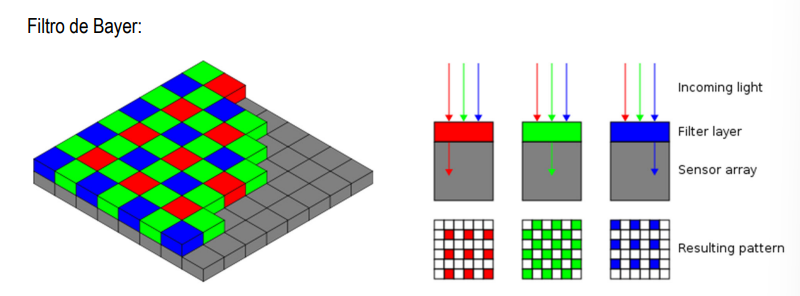
\includegraphics[width = \textwidth]{figs/filtro-bayer.png}
\end{figure}
La principal limitación de los CFA es que la resolución espacial de color es inferior a la resolución nominal del sensor. Para generar una imagen en color completa (donde cada píxel tenga valores R, G y B), es necesario aplicar un algoritmo de interpolación cromática o \textit{demosaicing}. Este proceso estima los componentes de color faltantes en cada píxel basándose en la información de los píxeles vecinos, lo que puede introducir artefactos como el \textit{moiré} o falseado de color (\textit{color aliasing}).
\end{itemize}

\section{Representación de imágenes}
\subsection{La imagen digital}
Una imagen digital es una representación bidimensional de una escena que ha sido \textbf{muestreada espacialmente y cuantificada en amplitud}. Esto significa que está definida en:
\begin{itemize}
\item Un dominio espacial discreto: un número finito de posiciones (píxeles) organizadas en una rejilla regular (matriz M×N).
\item Un rango de valores discreto: las intensidades solo pueden tomar un conjunto finito de valores (generalmente potencias de 2).
\end{itemize}

El \textbf{píxel} (elemento de imagen) es la unidad mínima de información espacial en una imagen digital. Cada píxel almacena un valor (o un conjunto de valores) que representa la intensidad luminosa y/o el color capturado por el sensor en esa posición específica. Así, una imagen digital puede representarse matemáticamente como una matriz de valores numéricos.

\subsection{True Color}
El término True Color se refiere a un método de representación de color que utiliza una codificación directa de los componentes cromáticos, típicamente capaz de representar más de 16 millones de colores distintos.

Es crucial hacer una distinción conceptual:
\begin{itemize}
\item \textbf{Imagen en Escala de Grises (Luminancia):} Se almacena un único valor por píxel, que representa la luminancia (la medida física de la intensidad de la luz), no la percepción subjetiva del brillo. Con una profundidad de 8 bits por píxel (bpp), se pueden representar 256 ($2^8$) niveles de gris, donde 0 suele representar el negro absoluto y 255 el blanco máximo.
\begin{figure}[h]
\centering
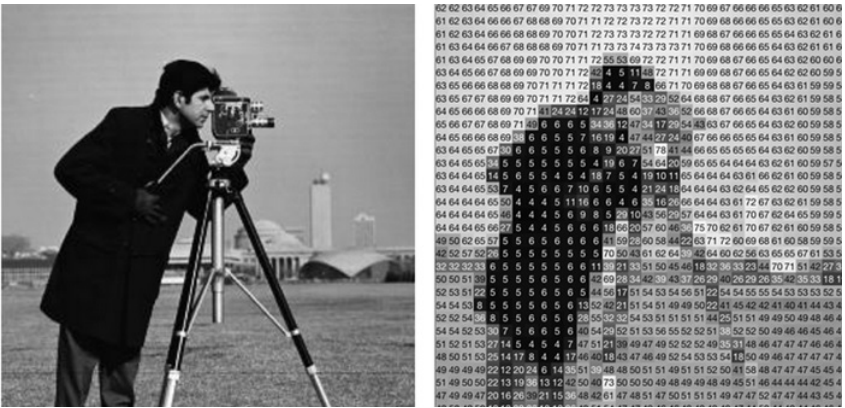
\includegraphics[width = 0.6\textwidth]{figs/true-color-mono.png}
\end{figure}

\item \textbf{Imagen True Color a Color}: Utiliza tres canales independientes (generalmente Rojo, Verde y Azul - RGB). Cada canal tiene una profundidad de 8 bits, resultando en un total de 24 bits por píxel (8 + 8 + 8). Esto permite representar $2^24 = 16.777.216$ colores distintos. Este tipo de imagen no es una matriz bidimensional simple, sino una estructura tridimensional de tamaño M×N×3, a menudo conceptualizada como "un cubo de información" donde cada "capa" corresponde a un canal de color.
\end{itemize}
\begin{figure}[h]
\centering
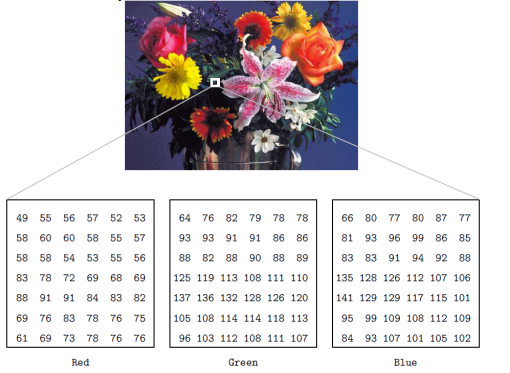
\includegraphics[width = 0.7\textwidth]{figs/true-color-tri.png}
\end{figure}

\subsection{Resolución vs definición}
La \textbf{resolución de la imagen (Pixel Dimensions}) se refiere al número absoluto de píxeles que componen la imagen en sus dimensiones de ancho y alto (e.g., 1920×1080 px). Es un atributo intrínseco del archivo digital y determina la cantidad de detalle espacial que la imagen contiene. El usuario puede seleccionarla durante la captura o el post-procesado (remuestreo).

La \textbf{Definición o Densidad de Píxeles (PPI - \textit{Pixels Per Inch} / DPI - \textit{Dots Per Inch})} es una medida de densidad que relaciona la resolución en píxeles con un tamaño físico real. Indica cuántos píxeles (PPI para pantallas) o puntos de tinta (DPI para impresión) hay en una pulgada lineal. Este valor define cómo de grandes o pequeños se verán los píxeles al reproducir la imagen en un dispositivo de salida (monitor, impresora). Está intrínsecamente ligado a la calidad del proceso de captura (óptica, sensor) y a las técnicas de procesamiento (interpolación, submuestreo) utilizadas.

\begin{figure}[h]
\centering
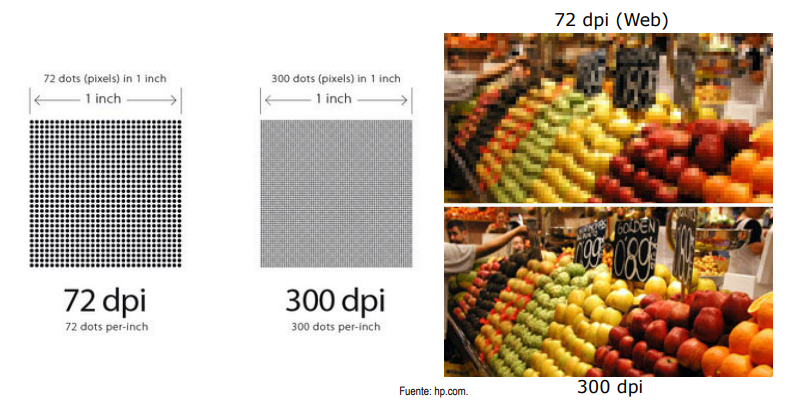
\includegraphics[width = 0.8\textwidth]{figs/resolucion-definicion.png}
\end{figure}

\subsection{Profundidad}
La profundidad de color se mide en bits por píxel (bpp) y determina cuánta información puede almacenar cada píxel, es decir, cuántos colores o tonos de gris diferentes puede representar una imagen.

\begin{figure}[h]
\centering
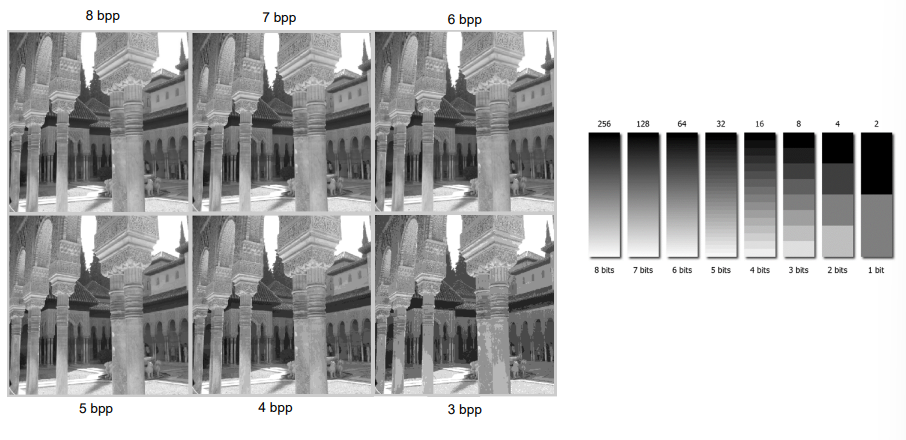
\includegraphics[width = 0.8\textwidth]{figs/profundidad.png}
\end{figure}

Aprovechando la menor sensibilidad del sistema visual humano a la información de color (crominancia) en comparación con la información de luminancia, se han desarrollado formatos que permiten comprimir imágenes reduciendo selectivamente los datos de color. Una alternativa al almacenamiento True Color (24 bpp) son las \textbf{imágenes indexadas}. En lugar de almacenar los tres valores RGB para cada píxel, se utiliza una paleta de colores o tabla de búsqueda (Color Look-Up Table - CLUT o Color Map). Esta paleta es un array de hasta 256 entradas (para 8 bpp) donde cada entrada contiene un color RGB de 24 bits.
La imagen en sí misma no almacena colores, sino índices (valores de 0 a 255) que apuntan a una posición en la paleta. Esto reduce drásticamente el tamaño del archivo. Se almacena una matriz de M×N de 8 bits (los índices) y una pequeña tabla auxiliar de 256×3 bytes (la paleta), en lugar de tres matrices de M×N de 8 bits.
No obstante, limita la imagen a un máximo de 256 colores simultáneos ($2^{nbits}$), lo que puede producir posterización (\textit{banding}) en imágenes con degradados suaves o muchas variaciones de color. Es ideal para gráficos con áreas planas de color.

\subsection{Formatos}
Hay muchos formatos de imagen:
\begin{itemize}
\item Sin compresión: BMP, RAW, PPM
\item Compresión sin pérdidas: PNG, GIF, TIFF
\item Compresión con pérdidas: JPEG, TIFF
\end{itemize}
%24/09 - Álvaro García
\chapter{Procesado imágenes digitales}
\section{Introducción}
El preprocesado y la mejora de imágenes tienen como objetivo:
\begin{itemize}
\item Realzar o mejorar el contraste.
\item Recortar (\textit{cropping}) o seleccionar regiones de interés.
\item Registrar: ajustar la geometría de una imagen para alinearla con otra.
\item Reducir o eliminar ruido y artefactos.
\item Corregir el desenfoque (\textit{deblurring}) o reconstruir áreas faltantes (\textit{inpainting}).
\end{itemize}

Un operador puntual se define de la siguiente manera:
Dada una imagen de entrada, el operador calcula cada píxel de la imagen de salida únicamente en función del valor del píxel en la misma posición (x, y) de la imagen de entrada, mediante una función matemática.

Un operador local, en cambio, calcula cada píxel de salida en función del píxel en la misma posición y de los píxeles de su vecindario en la imagen de entrada. La dependencia del vecindario está implícita en la función del operador.

\section{Operadores puntuales}
\subsection{Introducción}
Una transformación píxel a píxel donde el vecindario considerado es de 1x1, es decir, el propio píxel. Esto implica que las coordenadas espaciales del píxel son irrelevantes para la transformación. Se define como una transformación de los valores de intensidad de entrada, $r_k$, a valores de salida, $s_k$. Así, es un operador que modifica el nivel de gris de cada píxel individualmente. Estos operadores alteran la amplitud de los píxeles de acuerdo con una operación específica, lo que puede expandir la escala de grises para mejorar la visualización de detalles.

\begin{figure}[h]
\centering
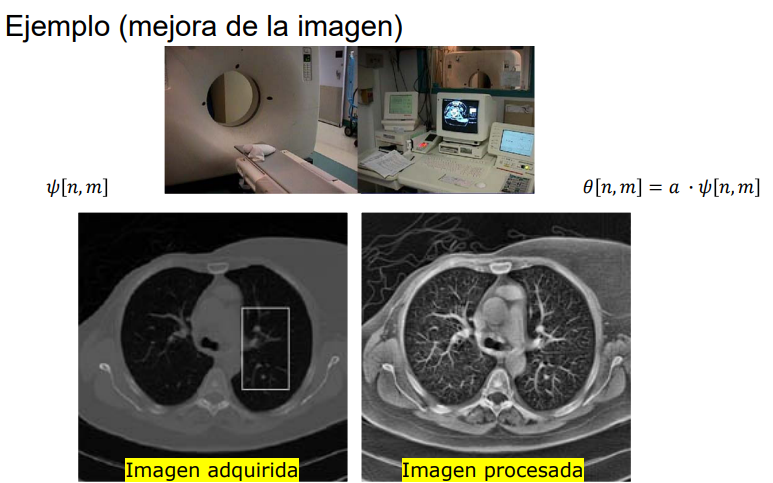
\includegraphics[width = 0.7\textwidth]{figs/mejora-puntual.png}
\end{figure}

\subsection{Modelado de histograma}
El histograma de una imagen $\psi[n,m]: h(r_k)$ denotado como $h(r_k)$, es una representación gráfica de la frecuencia de los niveles de gris. $h(r_k)$) indica el número de píxeles que tienen el valor $r_k$. 

Mientras la imagen original es bidimensional (coordenadas n, m), el histograma es unidimensional, ya que solo representa la distribución de frecuencias de los niveles de gris, sin información espacial.

\begin{figure}[h]
\centering
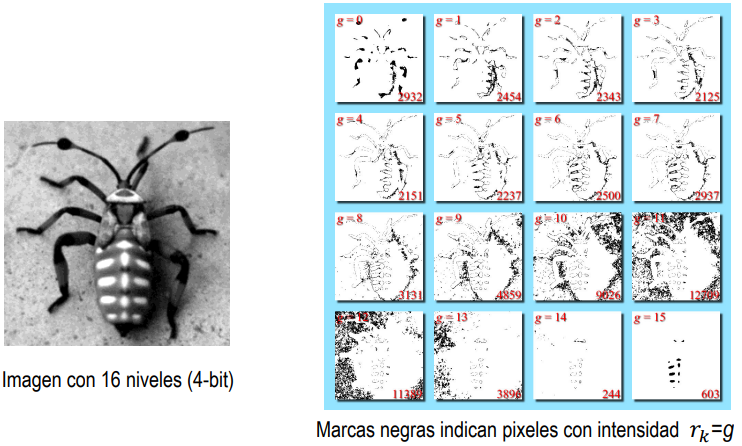
\includegraphics[width = 0.7\textwidth]{figs/histograma1.png}
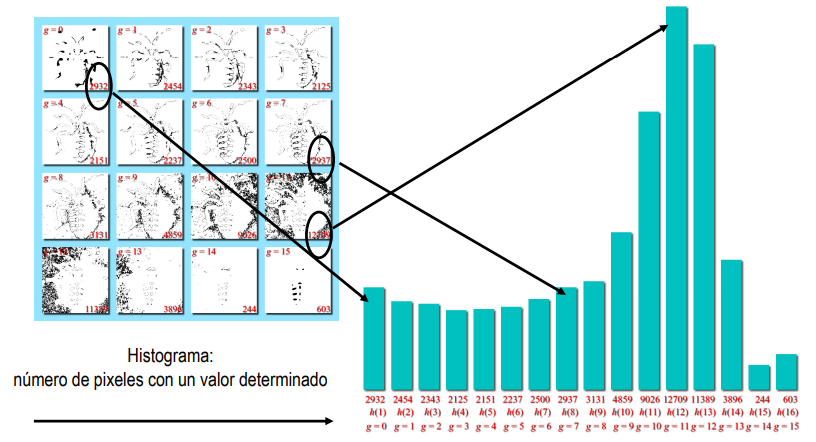
\includegraphics[width = 0.7\textwidth]{figs/histograma2.png}
\end{figure}

El histograma normalizado, obtenido al dividir cada valor del histograma por el número total de píxeles (ancho x alto de la imagen), estima la \textbf{función de densidad de probabilidad (FDP)} de los niveles de gris. La suma de todos sus valores es 1. Al acumular estos valores, se obtiene la \textbf{función de distribución acumulativa (FDA)} de la imagen, que siempre culmina en 1.

\begin{figure}[h]
\centering
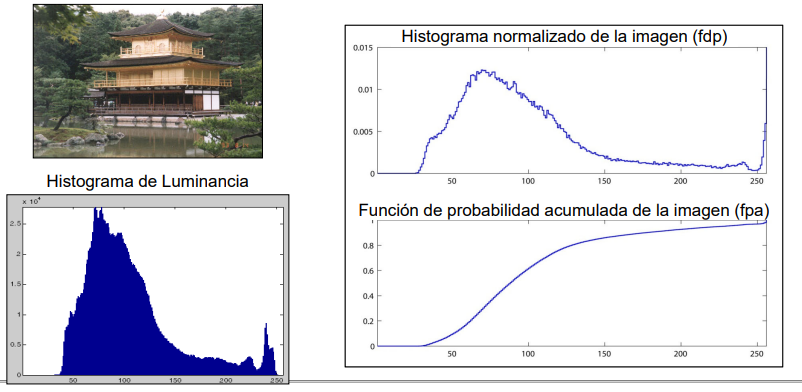
\includegraphics[width = 0.7\textwidth]{figs/fdp-fpa.png}
\end{figure}

Una limitación importante del histograma es que \textbf{no contiene información espacial} sobre la disposición de los píxeles en la imagen.

\subsubsection{Ajuste de contraste}
El objetivo es realzar imágenes con bajo contraste, causado por condiciones de baja iluminación, un rango dinámico limitado del sensor o errores en la configuración de la cámara (como la apertura del diafragma). La solución consiste en expandir o comprimir el rango dinámico de las intensidades según sea necesario.

Para expandir el contraste, se asigna un rango más amplio de valores de salida a un rango estrecho de valores de entrada en el histograma. Para reducir el contraste, se hace lo contrario. El objetivo es aprovechar todo el rango disponible de niveles de gris.

\begin{figure}[h]
\centering
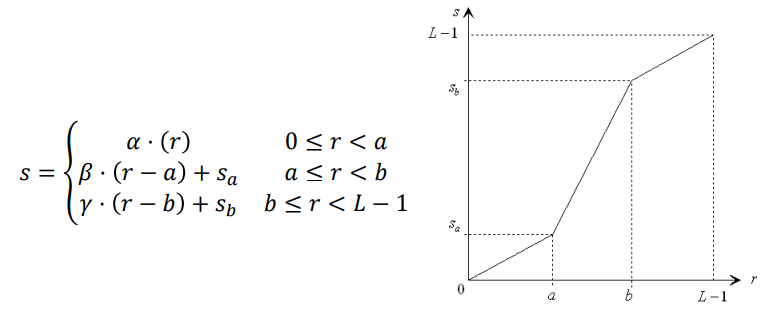
\includegraphics[width = 0.7\textwidth]{figs/ajuste-contraste.png}
\end{figure}

\begin{figure}[h]
\centering
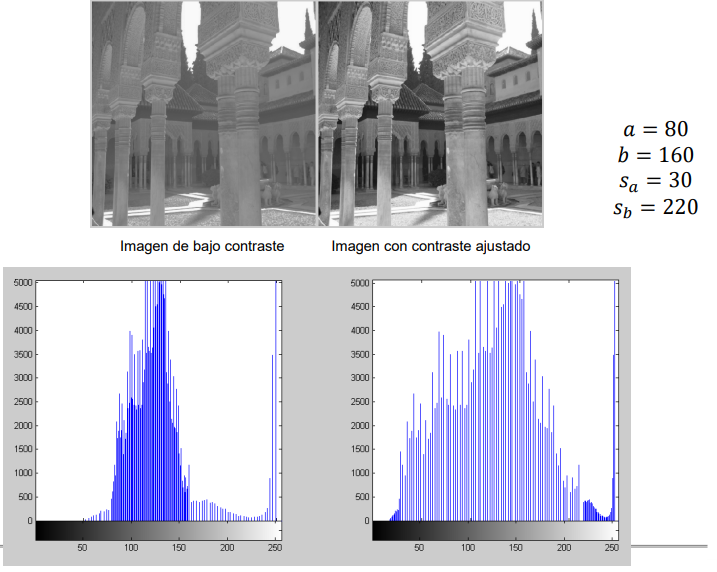
\includegraphics[width = 0.6\textwidth]{figs/ajuste-contraste-ej.png}
\end{figure}

En el ejemplo, un valor de entrada de 80 se transforma en 30, y un valor de 160 en 220. Esto expande el rango central de intensidades y comprime los extremos, logrando una mejor distribución del contraste.

\subsubsection{Igualación o ecualización (\textit{equalization)}}
La ecualización busca que la imagen resultante tenga un histograma lo más uniforme posible, es decir, que todos los niveles de gris tengan una frecuencia similar. Para ello, se utiliza la función de distribución acumulativa (FDA) del histograma normalizado como función de transformación. El efecto es una mejora continua y automática del contraste, a diferencia del ajuste por tramos.

\begin{figure}[h]
\centering
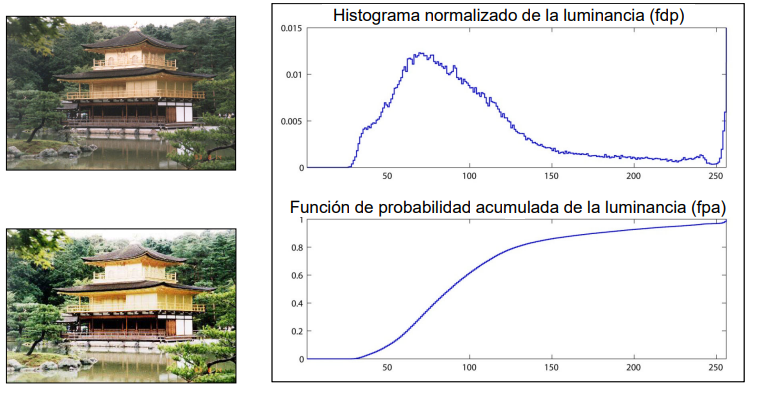
\includegraphics[width = 0.6\textwidth]{figs/equalization1.png}
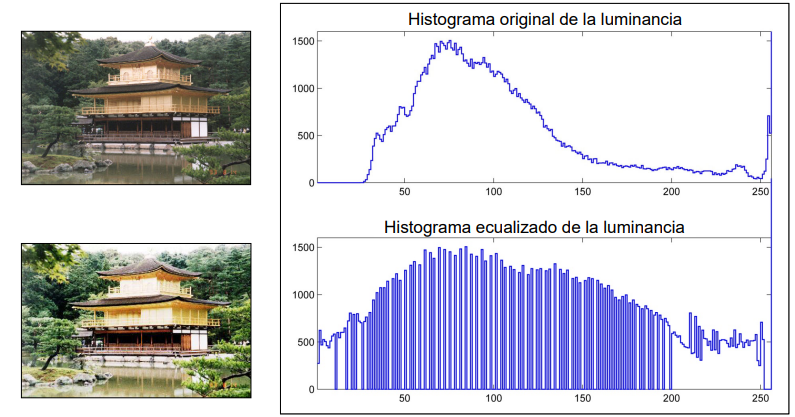
\includegraphics[width = 0.6\textwidth]{figs/equalization.png}
\end{figure}

La nueva intensidad de un píxel se calcula aplicando su FDA al rango máximo de grises (ej., 255). Por ejemplo, si la FDA de un nivel de gris es 0.6, su nuevo valor será $0.6 \cdot 255 \approx 153$.

\subsection{Modificación de niveles}
Estas técnicas permiten seleccionar información específica o crear efectos especiales modificando el histograma indirectamente. Los tipos principales son:
\begin{itemize}
\item \textbf{Recorte (\textit{clipping}):}

Similar al ajuste de contraste, pero "recorta" los valores por encima y por debajo de unos umbrales, asignándoles el valor máximo o mínimo. Las pendientes fuera del rango de interés se vuelven cero. Es útil para aislar regiones de interés o eliminar ruido cuando se conoce el rango válido de intensidades.

\begin{figure}[h]
\centering
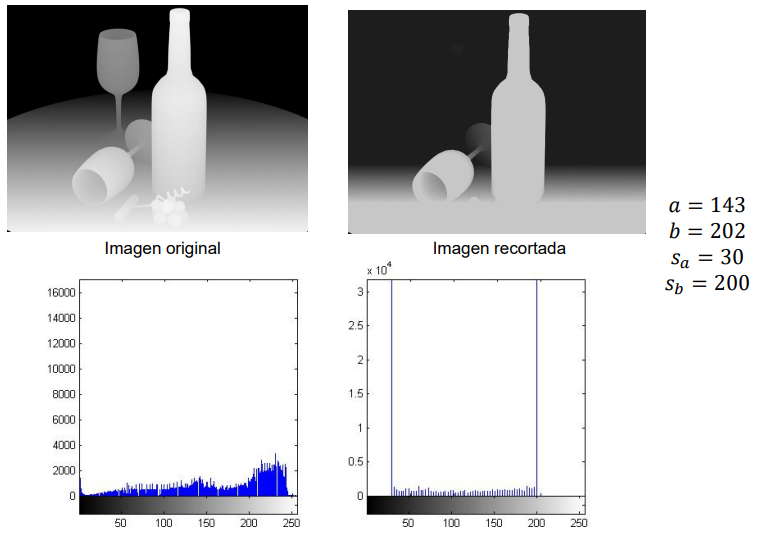
\includegraphics[width = 0.6\textwidth]{figs/recorte.png}
\end{figure}

Se utiliza, por ejemplo, en sistemas de ayuda a la conducción para ignorar obstáculos lejanos, o en robótica para limitar la percepción a distancias relevantes.

\item \textbf{Negativo o Inversión del eje de intensidades}:

Invierte los valores de intensidad (el blanco se vuelve negro y viceversa). Es útil en el análisis de imágenes médicas, como radiografías, para cambiar la perspectiva visual. El histograma resultante es la imagen especular del original.

\item \textbf{Seccionado de niveles (\textit{slicing}):}

Busca aislar una banda específica de niveles de gris, ya sea para extraerla o para resaltarla sobre el fondo.

\begin{figure}[h]
\centering
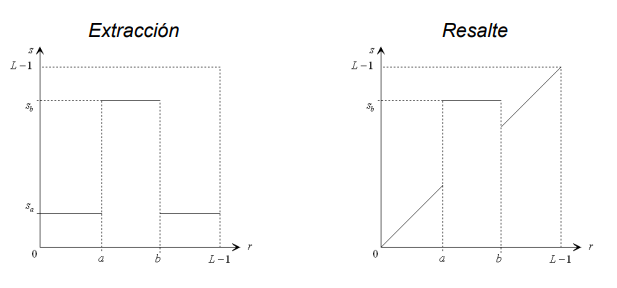
\includegraphics[width = 0.7\textwidth]{figs/extraccion-resalte.png}
\end{figure}

\begin{figure}[h]
\centering
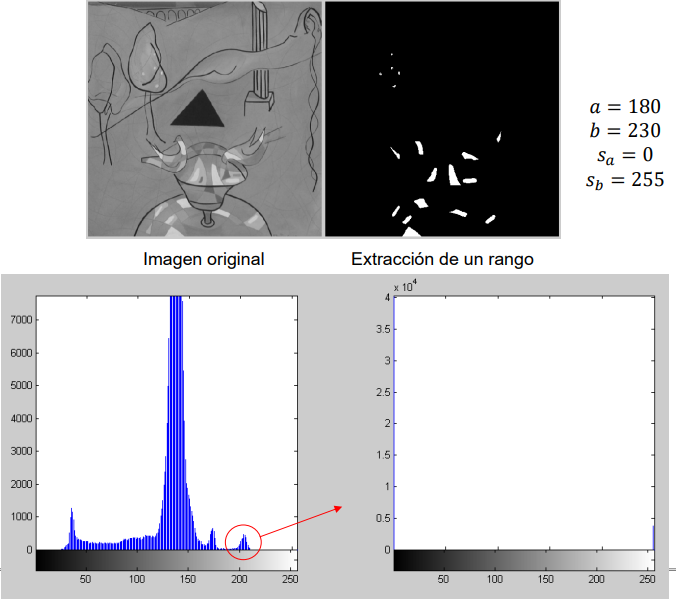
\includegraphics[width = 0.5\textwidth]{figs/extraccion-ej.png}
\caption{Ejemplo de extracción. Los píxeles dentro del rango seleccionado se muestran en blanco; el resto en negro.}
\end{figure}

\begin{figure}[h]
\centering
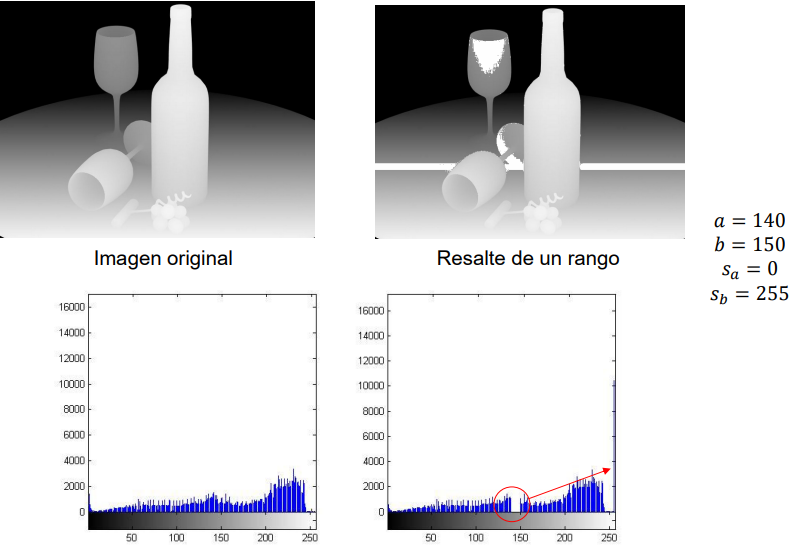
\includegraphics[width = 0.5\textwidth]{figs/resalte-ej.png}
\caption{Ejemplo de resalte. Una banda específica (ej., 140-150) se resalta en blanco. Puede usarse en sistemas de asistencia al conductor para marcar los límites de la distancia de seguridad.}
\end{figure} 
\end{itemize}

\section{Operadores locales}
Los operadores locales efectúan una transformación en el dominio espacial, conocida como \textit{filtrado espacial}.

\subsection{Filtrado espacial}
La operación de convolución se expresa como:
$$\theta [n,m] = \psi [n,m] \ast h[n,m] = \sum^a_{k=-1} \sum^b_{l=-b} \psi[k,l] \cdot h[n-k,m-l]$$

Para calcular $\theta[n,m]$, se centra la máscara invertida $h[-n,-m]$ sobre el píxel $\psi[n,m]$ y se calcula la suma de los productos de los píxeles de la vecindad por los coeficientes correspondientes de la máscara.

\begin{figure}[h]
\centering
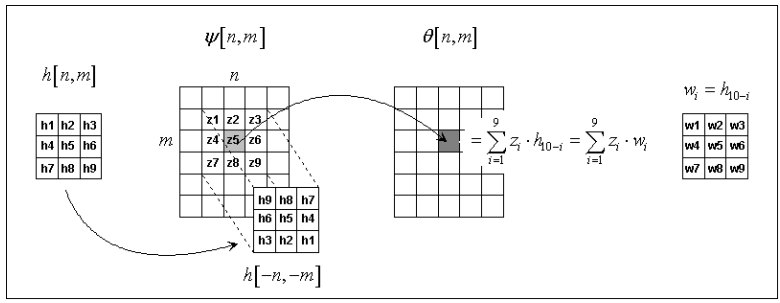
\includegraphics[width = 0.8\textwidth]{figs/convolution.png}
\end{figure}

La convolución de una imagen con un impulso (delta) desplaza la imagen. Por ejemplo, una máscara con un único '1' en una esquina desplazará la imagen. Si la máscara contiene varios impulsos, el resultado es una superposición de imágenes desplazadas y promediadas, lo que genera un efecto de emborronamiento.


Si en lugar de guardar solo 1 píxel de la matriz guardamos tres impulsos, se produce un desplazamiento y superposición. Se deben dividir entre 3 por normalización, y se guardan el píxel central, el píxel arriba a la izquierda y el píxel abajo a la derecha. Como se promedia, el resultado es una imagen movida emborronada.

Ahora guardamos 5 valores, las 4 esquinas y el valor central. La imagen resultante sigue estando movida. Esto se debe a que usualmente el vecindario no es tan grande. Si en lugar de utilizar un vecindario 16x16 se utiliza un vecindario 3x3, la convolución se convierte en un filtro de emborronado o suavizado que a simple vista no se aprecia, pero con zoom sí se aprecia que los bordes son más suaves al estar promediados.

En la práctica, se utilizan máscaras pequeñas (ej., 3x3). La convolución con una máscara de promediado produce un suavizado o desenfoque, haciendo los bordes menos nítidos.

Un desafío al aplicar convoluciones es el tratamiento de los bordes, donde la máscara se extiende más allá de la imagen. Las estrategias comunes para manejar esto son:
\begin{itemize}
\item \textbf{Relleno de ceros (\textit{Zero padding}):} Los píxeles fuera de la imagen se consideran 0.
\item \textbf{Réplica de píxeles (\textit{Replication}):} Se replican los valores de los píxeles del borde. Esta opción suele preferirse en imágenes médicas.
\item \textbf{Convolución circular:} La imagen se trata como periódica, tomando píxeles del lado opuesto.
\end{itemize}

\subsection{Suavizado: lineal y no lineal}
Los filtros de suavizado se utilizan para reducir ruido o difuminar detalles. En los filtros lineales, los coeficientes de la máscara son positivos y suman 1 para mantener el nivel de brillo promedio.

Los diseños comunes incluyen:
\begin{itemize}
\item \textbf{Filtro de media (\textit{averaging}):} Todos los coeficientes de la máscara son iguales.
\item \textbf{Filtro de media ponderada (\textit{weighted average}):} Los coeficientes son mayores en el centro, dando más peso al píxel central y a sus vecinos más cercanos. Un caso particular es el filtro binomial, que es separable y produce un suavizado más gradual.
\end{itemize}

La máscara de filtrado promediado ponderada es un caso particular de filtro binomial, familia de filtros separables resultante de la aplicación sucesiva y en ambas dimensiones de la máscara. El promediado da un resultado más borroso que el binomial.

El filtrado no lineal no se basa en una suma ponderada. Preserva mejor los bordes y es efectivo contra ruido impulsivo (como ruido sal y pimienta). Un caso paradigmático es el filtro de mediana, que reemplaza el valor del píxel central por la mediana de los valores en su vecindario. Otros filtros de estadísticas de orden son el de mínimo y el de máximo.

Filtro de mediana: en lugar de mezclar por igual, se aplica la función de la mediana. Se define un píxel central y un vecindario, y al vecindario se aplica la mediana. Eso mismo se puede hacer con el valor mínimo (filtro de mínimo), máximo (filtro de máximo) y filtro de posición. El filtro de mediana funciona muy bien para el ruido de sal-pimienta (puntos blancos y negros aleatorios). 

\begin{figure}[h]
\centering
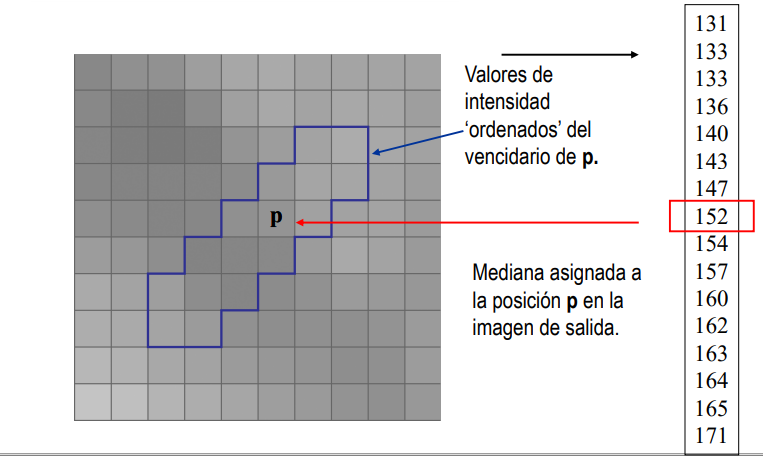
\includegraphics[width = 0.6\textwidth]{figs/filtro-median.png}
\end{figure}

\begin{figure}[h]
\centering
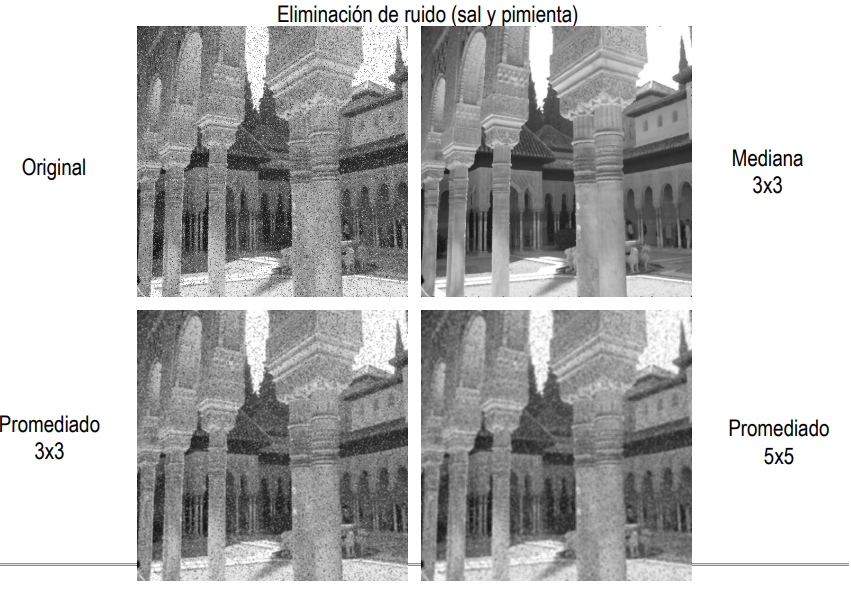
\includegraphics[width = 0.6\textwidth]{figs/sal-pimienta.png}
\end{figure}

\subsection{Realce: lineal}
Los filtros de realce resaltan detalles finos y bordes. Mientras el suavizado se asocia con la integración (promediado), el realce se relaciona con la derivación, que responde fuertemente a las discontinuidades (bordes) y al ruido.

En imágenes discretas, las derivadas se aproximan mediante diferencias. La primera derivada se implementa típicamente calculando la magnitud del gradiente. Los operadores más comunes para esto en máscaras 3x3 son los operadores de Prewitt, Sobel y Roberts.

El \textbf{operador de Prewitt} es un filtro de derivada parcial utilizado para calcular una aproximación del gradiente de la imagen en cada punto, lo que permite resaltar los bordes. Se compone de dos máscaras o kernels 3x3: una para calcular la derivada en la dirección horizontal (Gx) y otra para la dirección vertical (Gy).

\begin{figure}[h]
\centering
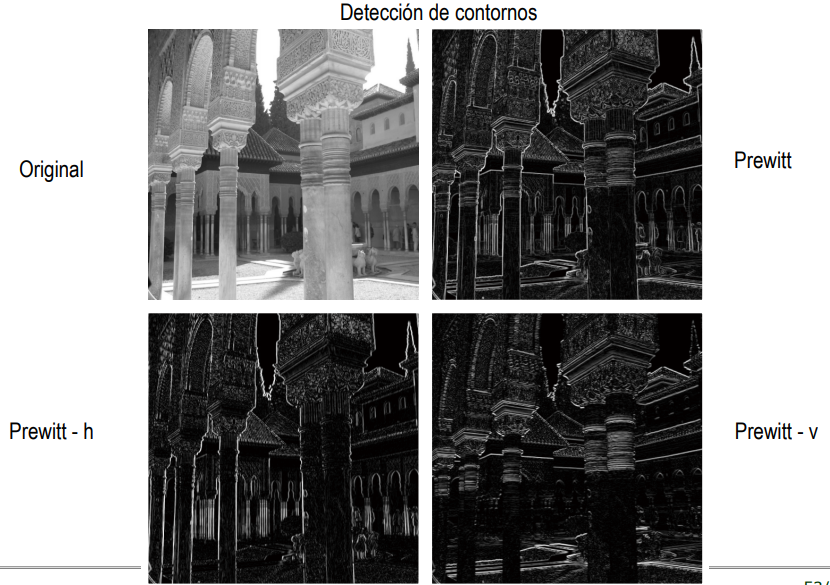
\includegraphics[width = 0.6\textwidth]{figs/prewitt.png}
\end{figure}
%29/09 - Blanca
\chapter{Registro de imágenes}
El registro de imágenes hace referencia a alinear en un mismo sistema de coordenadas unas imágenes. Esto tiene varias aplicaciones. Si en un mismo sujeto adquieres varios tipos de imagen en distintos puntos temporales, se puede alinear para ver la evolución temporal de esa zona. También se puede hacer entre sujetos para automatizar un estudio. Además, cada tipo de imagen médica (TAC, PET) puede proporcionar una información distinta, por lo que al alinearlo se puede tener una visión más completa. Por todo esto, el proceso de alinear imágenes es diferente en función de lo que se quiera conseguir. Así, los tipos de abordajes de registro depende de lo que se busque. En general, se busca minimizar la diferencia entre la imagen de entrada y la salida, o maximizando la similitud. 

\section{Tipos de registro}
Hay distintos tipos de registro:
\begin{itemize}
\item \textbf{Registro rígido}: El registro rígido solo permite rotar, manteniendo distancias y ángulos, y mover en el plano.
\item \textbf{Registro de similaridad}: Se añade un multiplicador de escala. Puede rotar, mover y ampliar. Esta transformación escala todas las direcciones en la misma medida, conserva los ángulos y las proporciones relativas, e incluye rotación y traslación.
\item \textbf{Transformación afín:} Además de todo lo anterior, permite el shearing, que es la alteración de la imagen al modificar un solo eje. Mientras que el escalado mantiene la forma, el shearing no. No es uniforme, ya que puede tener distintas escalas en cada eje.

\begin{figure}[h]
\centering
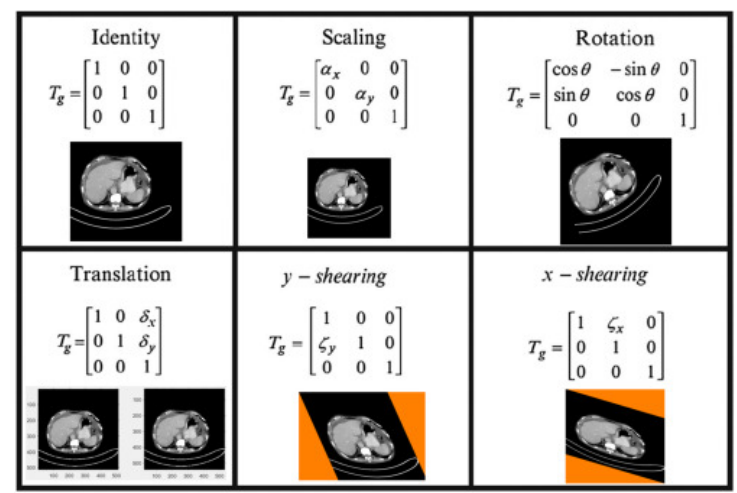
\includegraphics[width = 0.7\textwidth]{figs/registration.png}
\end{figure}

\item \textbf{Registro deformable:} Permite deformaciones locales que puede ser distinto para cada píxel. 
\item \textbf{Registro longitudinal:} Alinea múltiples imágenes del mismo sujeto a lo largo del tiempo, y puede seguir un registro rígido o deformable dependiendo de si se deben detectar cambios sutiles sin introducir deformaciones artificiales.
\item \textbf{Registro multimodal:} Alinea imágenes obtenidas mediante diferentes técnicas de imagen, como la resonancia magnética (estructural) y la tomografía por emisión de positrones (funcional). Las diferentes modalidades pueden tener contrastes distintos; entre las métricas de similitud comunes se incluyen la información mutua y la correlación cruzada. El registro multimodal preciso es fundamental para fusionar la información anatómica y molecular (por ejemplo, planificación quirúrgica, localización de tumores).
\end{itemize}

\begin{figure}[h]
\centering
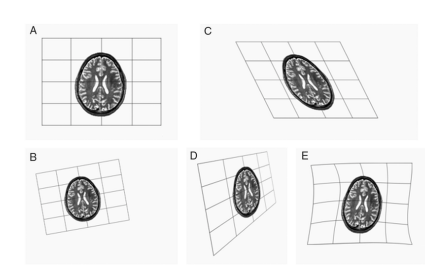
\includegraphics[width = 0.7\textwidth]{figs/registration-medical.png}
\caption{Un registro de imágenes médicas utilizando diferentes matrices de transformación. A) Una imagen original. B) Transformación de rotación y traslación. C) Transformación de rotación, traslación y cizallamiento. D) Transformación proyectiva. E) Transformación deformable.}
\end{figure}

\section{Avances clave en IA en registro de imágenes}
La IA está mejorando significativamente el registro y el co-registro de imágenes médicas al hacer que el proceso sea más rápido, más preciso y más robusto en entornos clínicos y de investigación.

Los modelos de aprendizaje profundo, como las redes neuronales convolucionales (CNN) y los modelos basados en transformadores, han revolucionado el registro de imágenes al aprender directamente cómo alinear imágenes a partir de ejemplos, saltándose el complejo diseño manual de características y la optimización iterativa.

Las arquitecturas CNN, como U-Net, predicen campos de deformación densos que describen los desplazamientos espaciales píxel a píxel necesarios para alinear las imágenes de forma rápida y precisa.

Los modelos basados en transformadores aportan la capacidad de aprender relaciones globales y dependencias contextuales en toda la imagen, lo que mejora la precisión del registro, especialmente en el caso de variaciones anatómicas grandes o complejas.

Los modelos de IA pueden realizar registros rígidos (traslación, rotación) y deformables (deformación no lineal), lo que ayuda a alinear órganos o tejidos que pueden haber cambiado de forma entre exploraciones.
 
A diferencia de los métodos de registro clásicos que se basan en procesos iterativos y métricas elaboradas manualmente, los algoritmos de IA realizan predicciones en un solo paso, lo que acelera enormemente el proceso de alineación y lo hace escalable para los flujos de trabajo clínicos.

Los enfoques de registro de IA se generalizan mejor en imágenes multimodales (por ejemplo, de PET a MRI) utilizando funciones de similitud aprendidas, superando las limitaciones de las métricas tradicionales basadas en la intensidad que tienen dificultades con los diferentes contrastes de las imágenes.

Estos avances permiten aplicaciones como la monitorización de la progresión de enfermedades, la planificación de tratamientos y estudios de investigación que requieren una alineación espacial precisa de grandes conjuntos de datos de imágenes.

\section{Artículo}
\textbf{Evaluación de un procedimiento de registro conjunto de imágenes multimodales (TC, RM y PET) en fantomas y pacientes con cáncer de cabeza y cuello: precisión, reproducibilidad y consistencia}

En el artículo busca mejorar la radioterapia en tumores. Se realiza una radiografía para ver el tumor y poder crear una terapia dirigida. Hay que tener en cuenta la intensidad de la radiación y la geometría del haz y dónde va a impactar en la anatomía del tumor. Para ello, se validan unas técnicas de corregistro entre distintas imágenes para delimitar lo mejor posible el volumen tumoral. Es un trabajo multi-técnica al utilizar PET (tomografía por emisión de positrones), TAC y resonancia magnética. Esto lo prueban en un phantom (tejido simulado para probar la técnica) y en pacientes. 

El objetivo del estudio era validar un método interactivo de corregistro rígido basado en segmentación de superficies para fusionar imágenes de CT, MRI y PET. Como sujetos se utilizaron fantomas diseñados con estructuras que simulan el cuello y 4 pacientes con carcinoma de células escamosas faríngeo-laríngeo.

Como referencia se utilizaba la tomografía computerizada (CT). Un observador ajustaba manualmente la traslación y rotación de una imagen sobre dicha referencia hasta lograr una superposición visual óptima. Los parámetros de transformación se guardaban.

El accuracy se definió como la diferencia entre la transformación aplicada por un observador y el valor promedio de todas las transformaciones realizadas por todos los observadores para la misma modalidad de imagen.
Se expresó como 2 desviaciones estándar de la distribución de las traslaciones y rotaciones. También se usó el vector euclidiano para combinar traslaciones en x, y, z y obtener un desplazamiento total en mm.

Se utilizó la reproducibilidad para medir cuán consistentes son los resultados cuando el mismo proceso lo realiza diferente gente o la misma persona en diferentes momentos. Se calculó la variación intra-observación (varianza de los resultados de corregistración de una misma persona 4 veces con días de separación) y variación inter-observador (4 observadores diferentes).  Se comparó esta varianza con la Varianza Residual (la varianza total que no se puede explicar por el observador), para ver si el factor "observador" era significativo.
Las variaciones intra e inter-observador fueron muy pequeñas (varianzas < 0.25 mm2) y muy inferiores a la varianza residual. Esto significa que el factor "observador" es insignificante y que cualquier clínico entrenado puede obtener resultados similares.

Finalmente, la consistencia medía si el método produce resultados coherentes cuando se aplica a diferentes tipos de imágenes del mismo sujeto. Para ello, se compararon los parámetros de coregistro obtenidos para las secuencias MRI T1 y MRI T2 de un mismo paciente. Como ambas se adquieren en el mismo equipo sin mover al paciente, deberían coregistrarse con los mismos parámetros. Cualquier diferencia indica una inconsistencia del método.
No hubo diferencias significativas al coregistrar MRI T1 vs. T2, excepto en una dirección (y), lo que sugiere que el método es robusto frente a cambios en el contraste de la imagen.

%Algunas imágenes son más anatómicas y otras más funcionales. Por ello, se distinguen imágenes de mapas. Los mapas se construyen a partir de varias imágenes. Las imágenes de difusión se utilizan mucho en clínica para procesos isquémicos en el cerebro. Mediante el movimiento de las moléculas de agua se puede ver el gradiente de los campos magnéticos para ver la estructura. Según la señal de resonancia magnética y las imágenes, se obtiene el valor de difusión a través de una fórmula matemática. Esto se registra y se construye un template. Los mapas se alinean con el template, el cual se debe bajar de resolución. 

\section{Imágenes, mapas y templates}
En el procesamiento de imágenes biomédicas conviene establecer una clara diferenciación entre lo que constituye una \textbf{imagen} y lo que representa un \textbf{mapa}. Las imágenes corresponden a datos directos adquiridos por los equipos de imagenología, como tomografías computarizadas, resonancias magnéticas o estudios de tomografía por emisión de positrones. Estos datos pueden presentarse en forma cruda o reconstruida, conteniendo información anatómica o funcional directa del paciente.

Por otro lado, los mapas representan datos derivados obtenidos mediante procesamiento matemático avanzado. Se construyen a partir de múltiples imágenes y encapsulan parámetros fisiológicos o físicos cuantitativos, proporcionando una representación numérica de propiedades tisulares específicas que no son directamente observables en las imágenes originales.

\subsection{Imágenes de Difusión en Neuroimagen}
Las imágenes de difusión por resonancia magnética se fundamentan en el movimiento browniano de las moléculas de agua en los tejidos biológicos. Desde la perspectiva física, esta técnica emplea gradientes de campo magnético específicamente diseñados para sensar el desplazamiento molecular. El movimiento de las moléculas de agua modula la señal de resonancia magnética de manera característica, permitiendo cuantificar las restricciones a la difusión mediante la atenuación de la señal observada.

En la práctica clínica, las imágenes de difusión han demostrado un valor incalculable para la detección de isquemia cerebral aguda. Durante un evento isquémico, se produce una restricción significativa de la difusión molecular que se manifiesta como una hiperintensidad característica en las imágenes ponderadas por difusión. Esta propiedad convierte a esta modalidad de imagen en una herramienta esencial para el diagnóstico temprano de accidentes cerebrovasculares, permitiendo intervenciones terapéuticas oportunas.

\subsection{Construcción de Mapas de Difusión}
La transición desde imágenes de difusión hacia mapas paramétricos implica un proceso de reconstrucción matemática sofisticado. El mapa de Coeficiente de Difusión Aparente (ADC) se obtiene mediante un ajuste por mínimos cuadrados realizado voxel por voxel, aplicando el modelo exponencial $S(b) = S(0) \cdot \exp(-b \cdot ADC)$, donde $S(b)$ representa la intensidad de señal con el gradiente de difusión aplicado, $S(0)$ denota la intensidad de señal sin gradiente de difusión, $b$ corresponde al factor de difusión expresado en $s/mm^2$ y $ADC$ simboliz el coeficiente de difusión aparente en $mm^2/s$.

El flujo de procesamiento comienza con la adquisición de múltiples imágenes de difusión utilizando diferentes valores del factor b. Posteriormente, se ejecuta la reconstrucción paramétrica mediante ajuste exponencial para generar el mapa de ADC voxel por voxel. La fase final incluye la validación y control de calidad del mapa resultante, asegurando la confiabilidad de las mediciones cuantitativas obtenidas.

\subsection{Registro de imágenes y templates}
En el contexto del análisis espacial estandarizado, los templates representan imágenes de referencia que definen espacios coordenados normalizados, como los sistemas MNI o Talairach. Estos templates poseen resoluciones espaciales predefinidas, típicamente de $1mm^3$ o $2mm^3$, y sirven como base fundamental para análisis multi-sujeto y comparaciones poblacionales.

El proceso de registro espacial implica la alineación geométrica de imágenes individuales con el template de referencia. Desde una perspectiva práctica, es la imagen individual la que normalmente se somete a re-muestreo para emparejar la resolución del template, estrategia conocida como \emph{downsampling}. Esta aproximación se justifica por el hecho de que los algoritmos de registro funcionan de manera óptima cuando las imágenes involucradas presentan resoluciones espaciales similares. Cabe destacar que en situaciones excepcionales donde el template presenta mayor resolución que la imagen individual, podría aplicarse el proceso inverso de \emph{upsampling}.
%01/10 
\chapter{Segmentación de imágenes}
\section{Introducción}
La segmentación de imágenes tiene como objetivo la partición de una imagen en regiones o segmentos homogéneos con respecto a alguna característica (color, forma, distancia, tamaño) con el fin de simplificarla e identificar elementos de interés para una aplicación concreta. Toda la imagen está segmentada y la unión de los fragmentos recupera por completo la imagen.

En medicina, las aplicaciones de la segmentación incluyen la detección del borde coronario en angiogramas, medición del volumen tumoral y su respuesta a la terapia, mapeo funcional, clasificación automatizada de células sanguíneas, detección de microcalcificaciones en mamografías, extracción de imágenes del corazón a partir de cineangiogramas cardíacos, detección de tumores, etc.

La región $\Omega_j$ se define por un conjunto de píxeles "similares" de acuerdo a alguna característica definida sobre los píxeles de la imagen. 

Al medir la luminancia y conectividad, se miden si los píxeles se tocan (son conexos) o no (están segmentados). En una conectividad de 4, los píxeles que son conexos son los de arriba y abajo con respecto al píxel en cuestión, mientras que una conectividad de 8 implica que todos los de alrededor (incluidos los de la diagonal) son conexos. La luminancia y conectividad nos permiten diferenciar correctamente.

\begin{figure}[h]
\centering
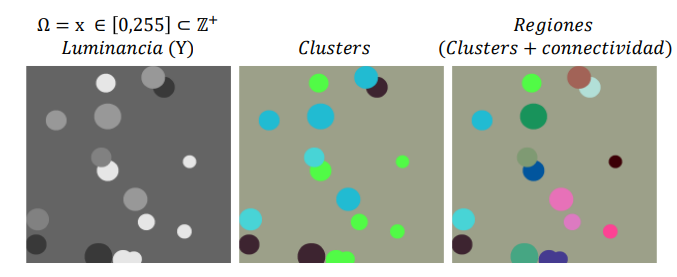
\includegraphics[width = 0.8\textwidth]{figs/luminancia-conectividad.png}
\end{figure}

Se utiliza una \textbf{etiqueta o label} como identificador de la región en la segmentación. Puede tener un número o color aleatorio y simplemente indica las regiones independientes y por tanto diferentes a las demás. 

Un \textbf{representante} es un descriptor de las características de la región de igual dimensión (d) que el espacio de decisión. Se realiza la estadística de lo que se quiere representar (media, mediana, moda). 

El \textbf{contorno} se define como el conjunto de píxeles alrededor de la región $\Omega_j$ en cuyo vecindario 9 hay al menos un píxel perteneciente a la región $j$ y un píxel no perteneciente a la región $j$. 

Sin embargo, esto está mal condicionado, ya que no hay un criterio para definir una región. Diferentes usuarios pueden considerar diferentes regiones y diferentes anotaciones. Además, el resultado depende de la escala y el conocimiento previo que se pueda tener ayuda a tomar las decisiones.

Hay distintos tipos de segmentación:
\begin{itemize}
\item \textbf{Clases:} separar objetos de su entorno, como por ejemplo separar una vaca del fondo de la imagen.
\item \textbf{Instancias:} separar  objetos individuales, para poder diferenciar por ejemplo dos personas juntas del fondo y entre ellas.
\item \textbf{Partes:} se identifican las distintas partes de los objetos
\item \textbf{Partes (alto nivel):} se siguen identificando las distintas partes de los objetos, pero sin tanto detalle, siendo así un punto intermedio entre instancias y partes.
\end{itemize}

\section{Técnicas más representativas}
Las técnicas más representativas se pueden clasificar en manual, semiautomáticas o automáticas, si son segmentación a bajo nivel o basada en modelo, o si son clásicas, basadas en estadísticos, difusas o redes convolucionales.

\subsection{Umbralización (operador puntual}
La umbralización o \textit{thresholding} es un caso particular de recorte para $a = b = T$. Así, la primera y última pendiente son nulas y la intermedia es absoluta. El threshold es un binario que divide la imagen en dos regiones, siendo así muy útil para imágenes bimodales.

Es útil para eliminar niveles cuando se sabe que el original sólo tiene dos y, en general, en la toma de decisiones binarias, como por ejemplo para finalizar la separación de objetos en procesos de segmentación.

\paragraph{Umbralización de imágenes bimodales}
Se utiliza un algoritmo que itera y, cuando la diferencia obtenida entre el nuevo umbral y el anterior es menor que la unidad, se detiene.

\paragraph{Método de Otsu}
Realiza una búsqueda exhaustiva del umbral que minimiza la varianza intra-clase. Busca el punto medio, pero teniendo en cuenta las distribuciones (variabilidad), permitiendo identificar objetos. 

\begin{figure}[h]
\centering
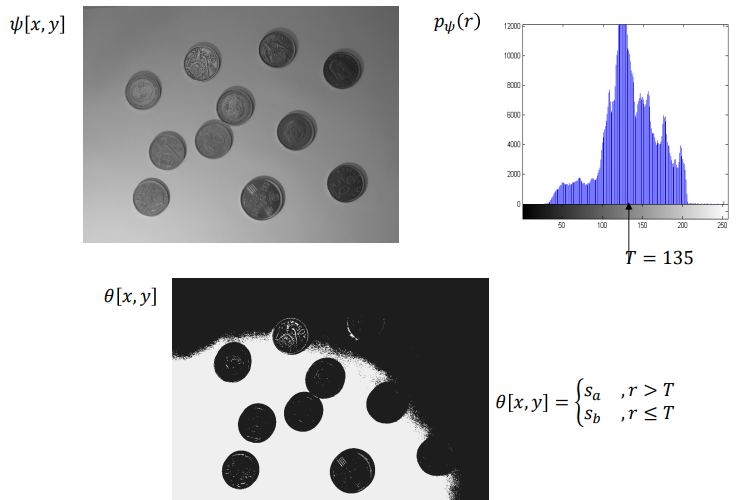
\includegraphics[width = 0.7\textwidth]{figs/umbralizacion-ej.png}
\caption{Si se utiliza la varianza para la umbralización, la imagen resultante (inferior) es muy mala al no realizar la separación entre fondo y monedas bien. Tanto la umbralización de imágenes bimodales como el método de Otsu son binomiales, y para este caso se debe segmentar en ventanas y aplicar la umbralización a cada ventana.}
\end{figure}

\begin{figure}[h]
\centering
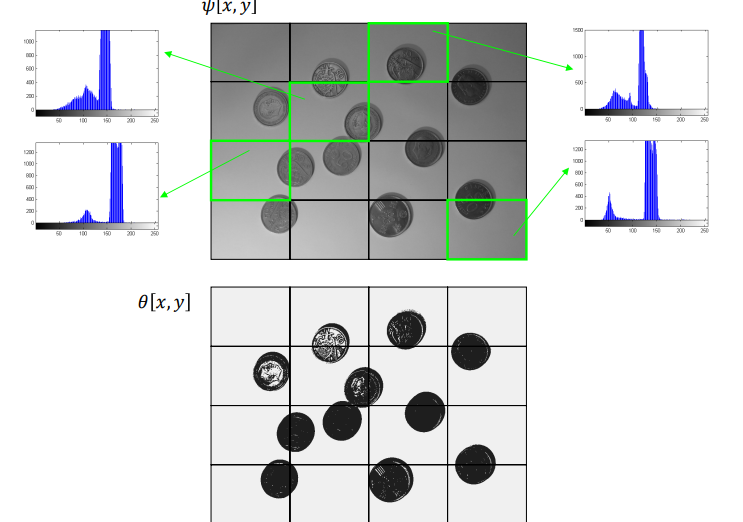
\includegraphics[width = 0.7\textwidth]{figs/umbralizacion-ej2.png}
\end{figure}

\paragraph{Multimodal} 
Para imágenes multimodales, se pueden aplicar los métodos anteriores bimodales repetidamente. De esta forma, primero se separan las dos regiones más grandes, y posteriormente de cada región se obtienen otras dos regiones contenidas en ella, etc. Esto se utiliza en la clasificación de tejidos mediante tomografía computarizada (CT). Mediante la consulta a expertos, se conoce la distribución y desviación de los tejidos. Estos datos se utilizan en algoritmos y se hacen medias dos a dos para poner un threshold.

\subsection{Clustering (agrupamiento por regiones)}
En el clustering, la imagen se divide entre K regiones más representativas. Las imágenes en color tienen un volumen de datos mayor, y el agrupamiento es díficil si se basa en el sistema visual humano.

Las aproximaciones son espacialmente "ciegas". La imagen se analiza como un conjunto de puntos d-dimensionales en el espacio de decisión. La técnica más representativa es \textbf{K-means}. Se busca la mejor frontera de separación entre los píxeles de sus vecinos más cercanos. 

Inicialmente hay tantos núcleos como píxeles. Cada núcleo tiene su celda, y se irán fusionando celdas si la distancia es menor que X. Esto se repite hasta obtener el número de clústeres que se quieran. El clustering clásico no tiene en cuenta el contorno, pero en imágnes RGB son 5 las variables que hay que tener en cuenta (rojo, verde, azul, x, y).
Los resultados dependen de la característica utilizada (feature space). Aunque nos regiones de la imagen sean del mismo color, se pueden segmentar en dos regiones utilizando similitud y proximidad.

El número de clústeres se escoge en función de lo que se busque ver.
\begin{figure}[h]
\centering
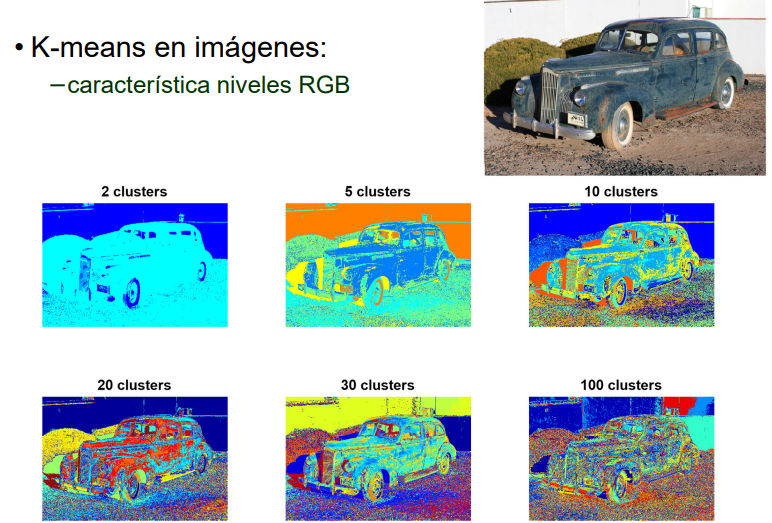
\includegraphics[width = 0.6\textwidth]{figs/clustering.png}
\end{figure}

\subsection{Detección y unión de bordes (basados en contornos)}
Se utiliza el detector de Canny, un algoritmo multietapa cuyo objetivo es localizar todos los bordes de una imagen con máxima precisión y sólo una vez cada borde. Las etapas se dividen en:
\begin{enumerate}
\item Suavizado de la imagen con un filtrado gaussiano. Esto sirve para que una imagen no se vea abrupta, sino continua.
\item Aproximación de la magnitud del gradiente y ángulo (Sobel/Prewitt).

Esto permite diferenciar los bordes en grados (ángulos de giro). Se hace la tangente y se calcula el ángulo. Saber el ángulo permite que, esté donde esté y tenga el grosor que tenga, se pueda obtener el punto medio analizando su perpendicular. 

\begin{figure}[h]
\centering
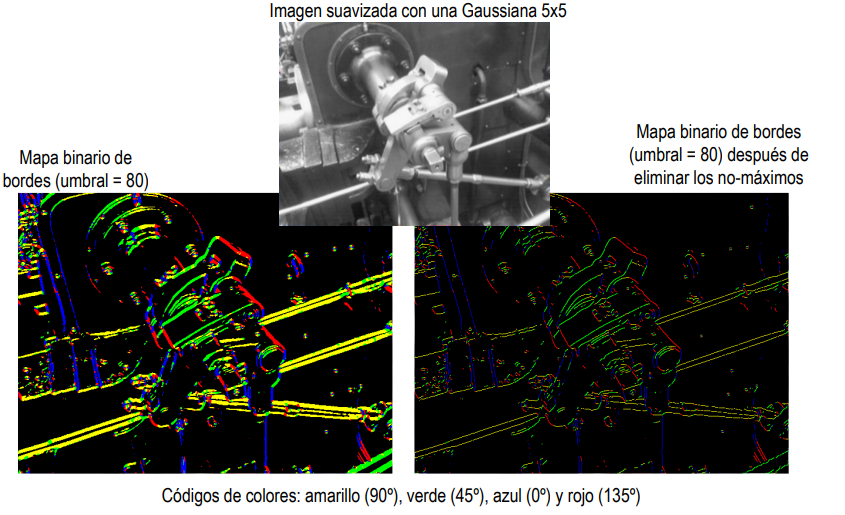
\includegraphics[width = 0.6\textwidth]{figs/deteccion-bordes.png}
\caption{La imagen izquierda tiene un grosor indefinido. La imagen derecha garantiza que todos tengan un borde de 1 píxel.}
\end{figure}

\item Umbralizado doble para detectar píxeles pertenecientes a bordes fuertes/débiles. Los bordes fuertes tienen grandes cambios de grises, mientras que los bordes suaves permiten cambios mínimos de grises.

\item Rechazo de píxeles en bordes débiles no conectados a bordes fuertes.
En el umbralizado alto, sólo se mantienen los bordes con cambios de gris muy exagerados de manera que hay granos de arroz que no terminan de asomarse.

\begin{figure}[h]
\centering
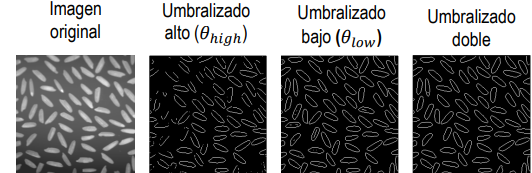
\includegraphics[width = 0.6\textwidth]{figs/bordes.png}
\end{figure} 
\end{enumerate}

\subsection{Contornos activos (basados en contornos)}
Los contornos activos snakes son un método global para la búsqueda de los contornos de los objetos en el espacio de decisión usando la imagen como soporte.

Es un proceso iterativo que busca rodear un objeto de interés, como puede ser un tumor. La snake se muestrea en un conjunto de puntos de control y busca minimizar una función de energía que combina:
\begin{itemize}
\item Energía interna: controla la deformación de la snake para evitar el sobreajuste.
\item Energía externa: controla el ajsute de la snake a los contornos para definir la calidad de la segmentación.
\item Energía restrictiva: restricciones de diseño, generalmente en función de la aplicación (ad hoc) o para incrementar la robustez al ruido.
\end{itemize}

El ajuste de snake se hace sobre una imagen de gradiente donde la curva tiende a meterse o salir del valle. Cuantas más iteraciones se hagan, mayor detalle se consigue.

\subsection{Redes convolucionales (deep learning)}
Las redes convolucionales (CNNs) son arquitecturas diseñadas para trabajar con datos estructurados espacialmente, como las imágenes médicas (microscopía, resonancia magnética, TAC, histología digital, etc.).

Un kernel (o filtro) es una pequeña matriz de pesos entrenables que se desplaza por la imagen (operación de convolución).
Cada kernel extrae un tipo de información: bordes, texturas, formas, o patrones más abstractos conforme se avanza en las capas.
Al principio, los kernels suelen detectar características de bajo nivel (bordes, contrastes), y en capas más profundas, rasgos de alto nivel (estructuras celulares, tejidos, órganos).

La idea es aplicar sucesivamente diferentes kernels entrenables de diferentes tamaños, diferentes niveles semánticos y combinar sucesivamente kernels a algunos más complejos.
Al aplicar convoluciones y pooling (submuestreo), la imagen va reduciendo su tamaño (se pierde resolución espacial). A cambio, las representaciones internas ganan en complejidad y profundidad: el número de canales (o mapas de características) aumenta. Esto genera un “código comprimido” de la imagen, útil para reconocer patrones globales.

\begin{figure}[h]
\centering
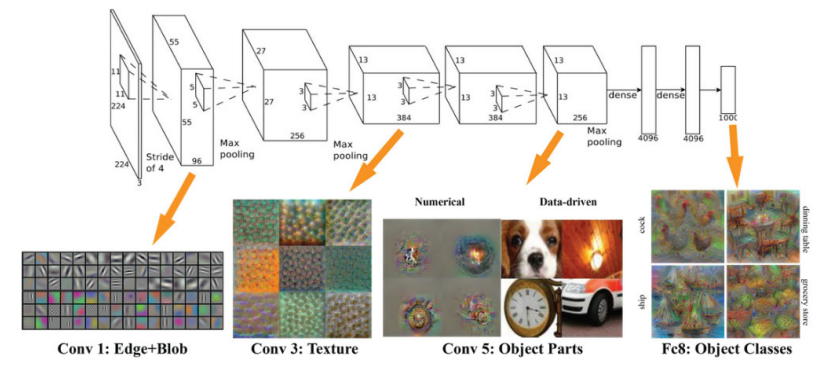
\includegraphics[width = 0.8\textwidth]{figs/convolutions.png}
\end{figure}

En clasificación, basta con decir si en la imagen hay un tumor o no. Pero en segmentación biomédica queremos una predicción a nivel de píxel (ej: qué píxeles son tumor, tejido sano, vasos sanguíneos, etc.). El \textbf{encoder} reduce la imagen extrayendo características relevantes. El \textbf{decoder} hace el proceso inverso, usando convoluciones transpuestas (deconvoluciones) o interpolaciones para recuperar la resolución original. Así, se obtiene un mapa de segmentación con la misma dimensión que la imagen inicial.

\begin{figure}[h]
\centering
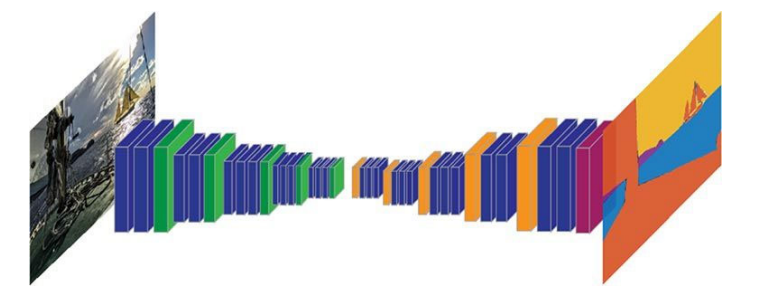
\includegraphics[width = 0.8\textwidth]{figs/encoder-decoder.png}
\end{figure}

%07/10 - Blanca Lizarbe
\chapter{Aplicaciones del Procesamiento Digital de Imágenes: CT, PET \& SPECT, Ultrasonido y Microscopía}
\section{Introducción y relación con la MRI}

La resonancia magnética (MRI) utiliza campos magnéticos y pulsos de radiofrecuencia, produciendo imágenes de tejidos blandos con alto contraste. Al igual que la MRI, la tomografía computarizada (CT) y la tomografía por emisión de positrones (PET) emplean reconstrucción tomográfica (a partir de información 2D se genera información 3D), aunque con diferentes fundamentos físicos y datos. Comprender los principios físicos de cada modalidad ayuda a anticipar los desafíos del procesamiento digital de imágenes. Una pregunta relevante sería: ¿qué características de las imágenes en el procesamiento de MRI se compartirán o diferirán en CT o PET? Todas son imágenes que se toman in vivo de todo el cuerpo. En cuanto al procesamiento, todos tienen el problema del movimiento, teniendo que corregir los artefactos de movimiento. PET tiene una resolución espacial más grande, por lo que el movimiento puede notarse menos, pero sigue afectando. En resonancia, hay un sesgo por el campo no ajustado. Los tipos de sensores que utilizan CT y PET tienen que sentir una radiación, teniendo otro tipo de sensibilidad.

\section{Tomografía Computarizada (CT/TAC)}

La CT utiliza una fuente de rayos X que rota alrededor del paciente, y los detectores miden la atenuación de los rayos X al atravesar los tejidos. Cada píxel de la imagen corresponde a una unidad de Hounsfield (HU) que representa la densidad del tejido.

En cuanto a las técnicas de reconstrucción, la retroproyección filtrada (FBP) aplica la transformada de Radon inversa para reconstruir la imagen a partir de proyecciones, mientras que los métodos iterativos mejoran el control del ruido y los artefactos, especialmente en exploraciones de baja dosis.

\begin{figure}[h]
\centering
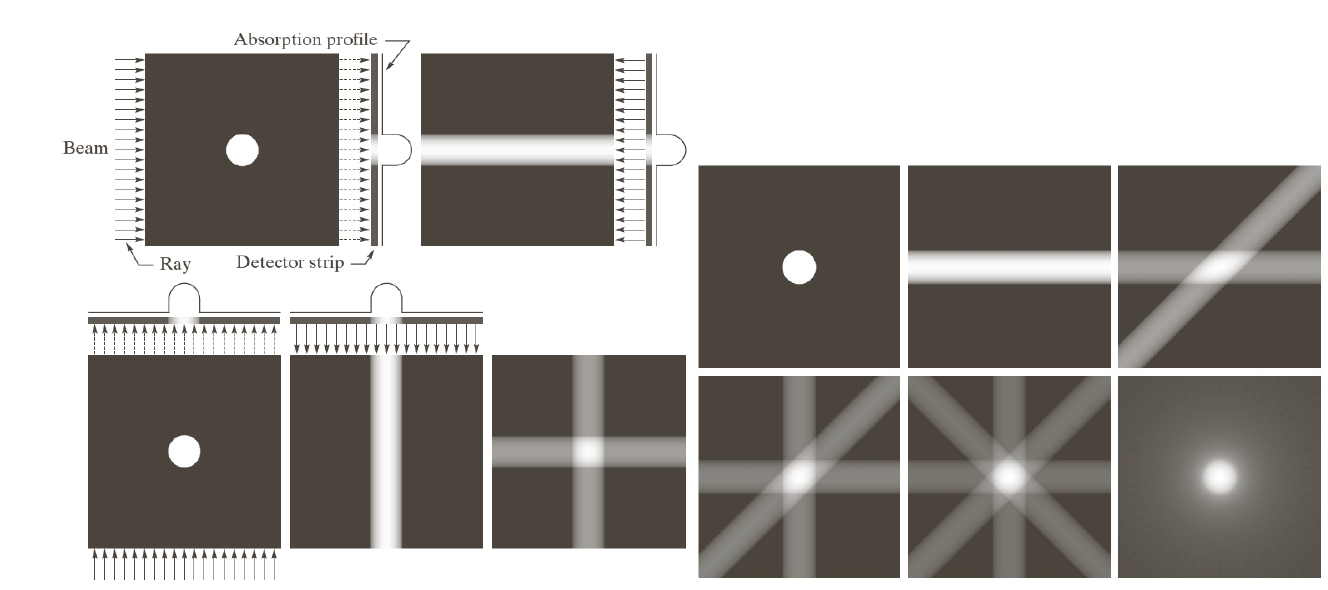
\includegraphics[width = 0.8\textwidth]{figs/backprojection.png}
\end{figure}

Las imágenes de CT presentan un alto contraste entre hueso y tejido blando, pero suelen ser más ruidosas que las de MRI. Los artefactos más comunes incluyen el \textbf{endurecimiento del haz} o \textit{beam hardening}, la dispersión y los artefactos metálicos. El endurecimiento del haz ocurre cuando los rayos X de menor energía son absorbidos preferentemente por estructuras densas, como hueso o implantes metálicos, lo que altera la interpretación del detector y genera efectos como bandas o “oscurecimiento” central. 

\begin{figure}[h]
\centering
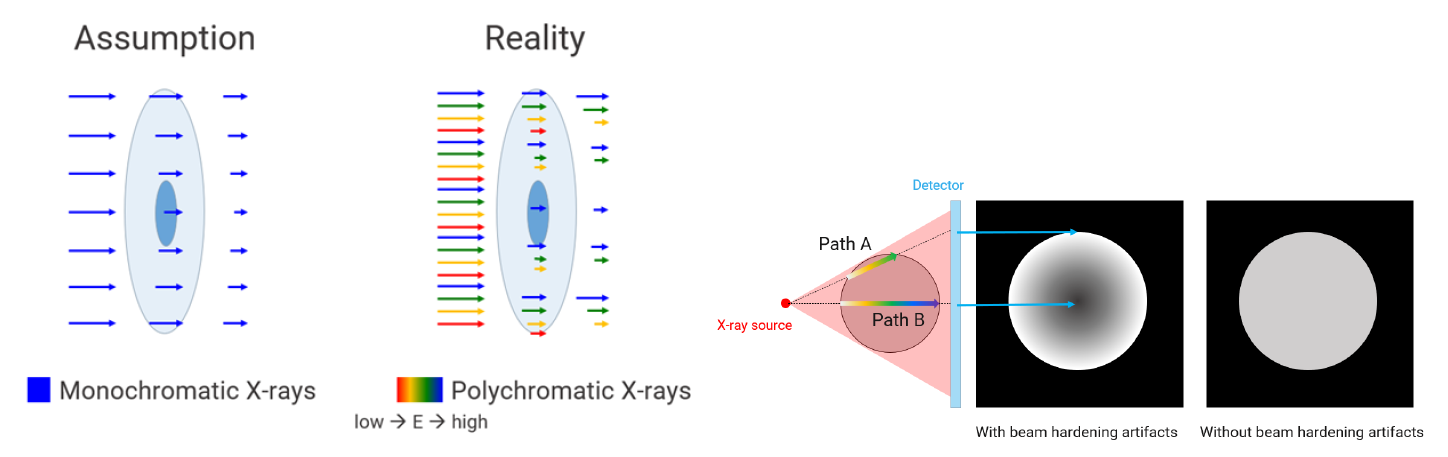
\includegraphics[width = \textwidth]{figs/beam-hardening.png}
\caption{La longitud del camino es corto para el camino A y largo para el B. Esto hace que haya menos endurecimiento del haz en el camino A y poca energía resultante de rayos X, además de alta tasa de absorción calculada y alta densidad reconstruida (claro). El camino B tiene más endurecimiento, mucha energía de rayos X, poco ratio de absorción calculado y poca densidad (oscuro).}
\end{figure}

La \textbf{dispersión}, causada principalmente por el efecto Compton, desvía los rayos X de su trayectoria, reduciendo el contraste y aumentando el ruido. Finalmente, los \textbf{artefactos metálicos} aparecen como bandas brillantes u oscuras alrededor de implantes metálicos.

El procesamiento de imágenes CT requiere preprocesamiento cuidadoso, reducción de ruido y artefactos. La segmentación enfrenta dificultades para diferenciar tejidos blandos y patológicos, y los datos volumétricos 3D exigen algoritmos eficientes para renderizado y análisis. Clínicamente, la CT se usa ampliamente en traumatismos, enfermedades pulmonares y óseas, y guía la planificación quirúrgica o de radioterapia. La física de la atenuación de rayos X influye directamente en los tipos de ruido y artefactos esperados.

\section{PET y SPECT}

La PET utiliza trazadores radiactivos que emiten positrones; estos se aniquilan con electrones, produciendo dos fotones de 511 keV detectados de forma coincidente por un anillo de detectores, permitiendo la reconstrucción tomográfica de la distribución del trazador, que refleja actividad metabólica o molecular. La SPECT, en cambio, usa trazadores que emiten fotones gamma simples, capturados mediante una cámara gamma que rota alrededor del paciente. Trazadores comunes incluyen Tecnecio-99m o Yodo-123. Las proyecciones obtenidas se reconstruyen en mapas tridimensionales mediante retroproyección filtrada o métodos iterativos.

La PET alcanza generalmente mayor sensibilidad y mejor resolución espacial que la SPECT, la cual está limitada por las estadísticas de fotones y la eficiencia del colimador. Ambas modalidades presentan un ruido considerable y baja resolución comparadas con CT o MRI, requiriendo algoritmos avanzados de corrección y eliminación de ruido. Las técnicas de aprendizaje profundo se aplican cada vez más para la mejora y reconstrucción de imágenes.

Debido al bajo conteo de fotones, las imágenes PET y SPECT suelen ser ruidosas, siendo SPECT la más afectada. La corrección por atenuación y dispersión es más compleja en SPECT, ya que depende de la emisión de fotones individuales y de la atenuación variable según los tejidos. Las imágenes PET y SPECT suelen fusionarse con exploraciones anatómicas (CT o MRI), lo que exige algoritmos de registro precisos para evitar desalineaciones que afecten la interpretación clínica. La segmentación y cuantificación presentan desafíos adicionales, como la definición precisa de regiones y la compensación de factores físicos y fisiológicos.

\begin{figure}[h]
\centering
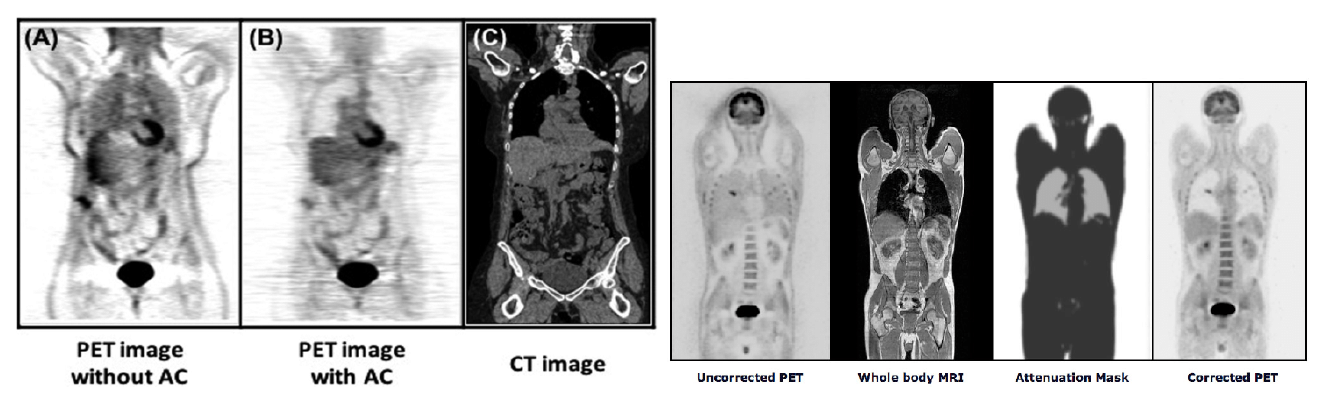
\includegraphics[width = \textwidth]{figs/atenuation-correction.png}
\caption{Corrección de atenuación (AC por sus siglas en inglés): A medida que los fotones emitidos por el trazador radiactivo viajan a través del cuerpo, algunos fotones son absorbidos o dispersados por tejidos como huesos, músculos o grasa. Esta pérdida de fotones significa que los detectores reciben menos fotones de los tejidos más profundos o densos, lo que hace que estas regiones parezcan artificialmente menos activas en las imágenes PET o SPECT.}
\end{figure}

En la práctica clínica, la PET se usa en oncología (detección y estadiaje tumoral), neurología (metabolismo cerebral) y cardiología (perfusión miocárdica). La SPECT se aplica en estudios de perfusión cardíaca, imagen ósea y cerebral, mapeo de receptores y diagnóstico de infecciones o inflamación. Aunque la resolución espacial es menor y tenga más artefactos y desventajas, su bajo costo y amplia disponibilidad de trazadores la hacen muy utilizada.

\section{Ultrasonido}

La ecografía utiliza ondas sonoras de alta frecuencia emitidas por un transductor, un dispositivo con un material que vibra con la electricidad para generar las ondas. Estas ondas viajan a través de los tejidos y se reflejan en las interfaces, siendo luego captadas y reconstruidas en imágenes en tiempo real. El proceso es altamente dependiente del operador y de las propiedades del tejido.

Uno de los principales desafíos del procesamiento de imágenes ecográficas es el ruido de moteado (\textit{speckle}), que surge por interferencia coherente de las ondas y genera un aspecto granular que reduce el contraste y dificulta la visualización de estructuras pequeñas. Se emplean algoritmos de eliminación de ruido especializados que preservan bordes y detalles finos.

\begin{figure}[h]
\centering
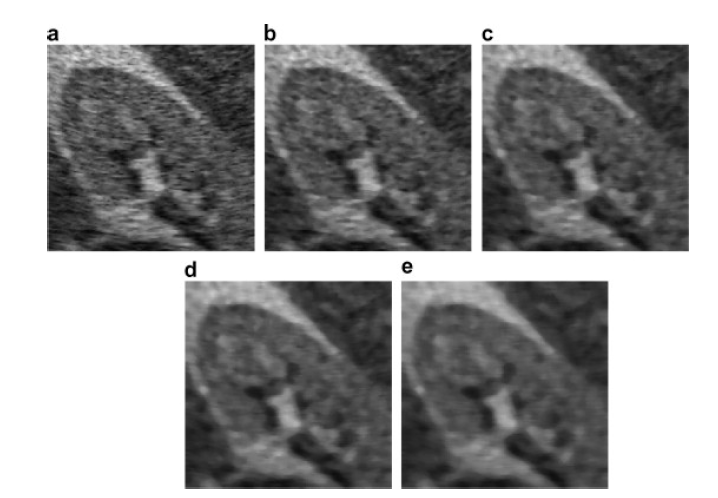
\includegraphics[width = 0.5\textwidth]{figs/speckle.png}
\end{figure}

La calidad de las imágenes varía considerablemente según el dispositivo, la habilidad del operador y la constitución del paciente. Los equipos portátiles suelen producir imágenes de menor calidad. Además, los artefactos como sombras, reverberaciones y efectos de atenuación dificultan la interpretación, por lo que deben detectarse y corregirse durante el procesamiento. Dado que el ultrasonido es una técnica dinámica y en tiempo real, los algoritmos de procesamiento deben ser rápidos y eficientes, equilibrando calidad de mejora y costo computacional.

\section{Microscopía}

La microscopía óptica captura las interacciones de la luz a escala micro o nanométrica, transformadas por sensores digitales en datos de píxeles. Las tareas de procesamiento incluyen corrección de enfoque automático, eliminación de ruido (especialmente en imágenes de fluorescencia con poca luz), y mejora de contraste o iluminación desigual. Los desafíos incluyen la calibración precisa para mantener la resolución espacial, la segmentación de células superpuestas y el manejo de grandes volúmenes de datos generados por la microscopía de alto rendimiento. En este contexto, se aplican métodos de aprendizaje profundo para la segmentación y eliminación de ruido, así como enfoques computacionales avanzados como la reconstrucción holográfica.

Las aplicaciones abarcan el conteo celular, el análisis morfológico, la patología, el cribado de fármacos y la investigación en biología molecular. Dada la variabilidad entre imágenes microscópicas, los pasos de preprocesamiento deben priorizar la corrección de iluminación, la normalización del color y la reducción de ruido antes del análisis cuantitativo.

\section{Integración y flujo de trabajo clínico}

Las modalidades de imagen suelen utilizarse conjuntamente, como en PET/CT o PET/MRI. Los flujos de trabajo automatizados incluyen reducción de ruido, registro y segmentación, apoyándose en estaciones centralizadas de procesamiento de imágenes médicas para la visualización multimodal. El éxito del procesamiento depende de comprender tanto la física de formación de cada modalidad como su contexto clínico.

\section{Conclusión}
\begin{itemize}
\item \textbf{CT:} Modalidad basada en rayos X que genera mapas tridimensionales de densidad. Los principales retos incluyen el ruido, artefactos como endurecimiento del haz o rayas metálicas, y la segmentación de tejidos blandos en presencia de estructuras de alto contraste.

\item \textbf{PET y SPECT:} Técnicas de medicina nuclear que miden la distribución funcional de trazadores. Presentan alto ruido por conteo limitado de fotones, correcciones complejas por atenuación y dispersión, necesidad de registro con CT o MRI, baja resolución y dificultades de análisis cuantitativo.

\item \textbf{Microscopía:} Imagen óptica de tejidos y células a micro/nanoescala, con retos de alta resolución, iluminación desigual, ruido en baja luz, segmentación compleja y grandes volúmenes de datos.

\item \textbf{Ultrasonido:} Imagen en tiempo real basada en ondas sonoras, afectada por ruido de moteado, variabilidad dependiente del operador y el equipo, artefactos de sombra y reverberación, y restricciones de procesamiento en tiempo real.

\end{itemize}

%08/10 - Álvaro
\chapter{Reconocimiento de patrones en imagen biomédica}
\section{Clasificación de imágenes}
\subsection{¿Qué es la clasificación?}
La clasificación busca asignar una etiqueta entre varias categorías o clases a una imagen o grupos de éstas. Se pueden asignar múltiples etiquetas a una imagen (multiestancia).

El algoritmo pasa primero por una fase de entrenamiento y una fase posterior de test e inferencia. El dataset es un conjunto de imágenes de entrenamiento (suele ser supervisado), que implica que el dataset viene etiquetado. Se extraen las características y se entrena con los datos de ejemplo y las etiquetas. De esta forma se obtiene un clasificador entrenado. 

En el test, se proporciona una imagen no existente en el entrenamiento. Se extraen las mismas características que se extrajeron en el entrenamiento aplicando el clasificador obtenido durante la fase de entrenamiento. Esto permite predecir la clase que hay en esa imagen.

\paragraph{Dataset} 
La base de datos se suele dividir en tres conjuntos para poder realizar validación cruzada. Las imágenes de entrenamiento sirven sólo para entrenar el clasificador. El subset de validación no sirve para entrenar, si no para medir el error y ajustar los parámetros. Las imágenes de validación nunca se deben usar para entrenar. Por último están las imágenes test, que dan una medida del error con datos nuevos que nunca se hayan visto. 

\paragraph{Extracción de características}
Las imágenes se deben modelar para extraer las características. Se pueden modelar los píxeles, histogramas de los niveles de gris, patrones (templates) o descriptores de regiones o puntos de interés entre otros.

\paragraph{Entrenamiento}
Se genera una función que obtiene una predicción al ser aplicada sobre características de la imagen.

\subsection{Evaluación del rendimiento}
La precisión de algoritmos de Machine Learning (ML) debe ser evaluada para seleccionar el mejor en cada tarea. 
Una tarea puede ser, por ejemplo, segmentación de tumores cerebrales en imágenes de resonancia magnética (MRI) e identificar qué píxeles son tumor.

Hay tres elementos clave para evaluar la efectividad de algoritmo (de clasificación) de manera sistemática:
\begin{itemize}
\item \textbf{Ground-truth/dataset}: valor o categoría real de cada dato para la tarea específica.
\item \textbf{Resultado}: predicción del algoritmo. Aunque se entrenen en otro dataset, deben ser evaluados en común. Esto significa que si entrenas un dataset de ayuda a la conducción con datos de Alemania, debe valer también para Suecia.
\item \textbf{Métrica}: función que calcula la similitud entre los valores o categorías del resultado y del ground-truth.
\end{itemize}

Hay diferentes modelos de entrenamiento en función de los distintos niveles de anotación. Un entrenamiento sin supervisión no está asociado a la etiqueta. Una supervisión débil define la clase o categoría, y una supervisión completa define los distintos segmentos. 

El resultado es la predicción del algoritmo. Tanto la predicción como el ground-truth son binarios, por lo que hay dos tipos de errores en clasificación: false negative y false positive. 
\begin{itemize}
\item Métricas focalizadas:

$$\text{precisión} = \frac{TP}{TP + FP} = \frac{correctos}{devueltos}$$

$$\text{sensitivity, recall, hit rate o true positive rate (TPR)} = \frac{TP}{TP + FN} = \frac{positivos}{total anotaciones positivos}$$

\item Métricas globales:

$$\text{Accuracy} = \frac{TP + TN}{TP + TN + FP + FN} = \frac{predicciones correctas}{total predicciones}$$

$$\text{Error rate} = \frac{FP + FN}{TP + TN + FP + FN} = \frac{predicciones incorrectas}{total predicciones}$$

$$\text{F-score} = 2 \cdot \frac{precision \cdot recall}{precision + recall}$$
\end{itemize}

Mediante una \textbf{matriz de confusión} se puede visualizar los aciertos y errores para clasificaciones multiclase.

\subsection{Clasificación basada en \textit{bag of words}}
Se aprenden diferentes características visuales que representen un objeto. El objeto se modela como mezcla de elementos básicos o textones. Dependiendo de su textura se van a agrupar de una forma u otra. La bag of visual words tiende a acumular los patrones más repetidos en un diccionario de textones y caracterizar en un histograma las veces que aparecen los textones en la imagen de entrada. No obstante, no se incluye información de localización espacial ni existe distinción entre frente y fondo de la escena, trata todas las texturas por igual. 

Son modelos para describir imágenes (contiene dos ojos, una nariz, una boca), pero no dónde se encontraba originalmente en la imagen (izquierda, derecha, arriba, centro, ...).

Las etapas del modelo son las siguientes:
\begin{enumerate}
\item Extracción de características de las imágenes
\item Aprendizaje del vocabulario visual
\item Cuantificación de características (palabras visuales) a partir del vocabulario visual; se puede limitar a un cierto número, como las 4 palabras visuales más clave, más frecuentes, más distribuidas, etc.
\item Representar imágenes como histogramas con palabras visuales
\end{enumerate}

\begin{figure}[h]
\centering
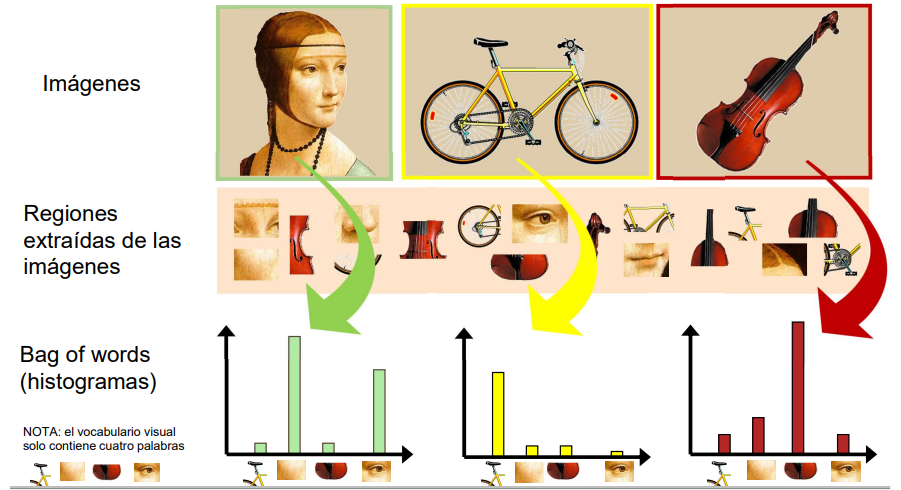
\includegraphics[width = 0.8\textwidth]{figs/bag-of-words.png}
\end{figure}

Este proceso se repite para cada imagen nueva que se encuentre. Todas las imágenes de entrada se matchean con el diccionario visual creado y se busca a la que más se parece. Una vez que se tienen los histogramas, se suele aprender un clasificador para distinguirlas.

\begin{table}[h]
\centering
\begin{tabular}{p{6.5cm}|p{6.5cm}}
Ventajas del modelo Bag-of-words & Desventajas del modelo Bag-of-words \\ \hline
Flexible a la geometría, deformaciones y puntos de vista & El fondo y el primer plano se mezclan al representar toda la imagen \\
Resumen compacto del contenido de la imagen & La formación óptima del vocabulario \\
Proporciona representación vectorial dimensional fija para conjuntos & El modelo básico ignora la geometría; debe verificarse después o codificarse mediante funciones \\
Muy buenos resultados en la práctica & 
\end{tabular}
\end{table}

\section{Detección de objetos}
\subsection{¿Qué es la detección de objetos?}
La detección de objetos permite clasificar y localizar objetos espacialmente en la imagen que discriminen la información del objeto de la información del fondo. La detección de objetos no es la identificación de objetos concretos, si no la clasificación de distintas clases de objeto genéricas.

Presenta muchos desafíos. En el caso de las personas, cada objeto tiene mucha variabilidad: la postura, altura, edad, escala, relación de aspecto, punto de vista más lejano, multitudes, iluminación, ropa. Esto dificulta identificarlos entre ellos.

Entre los criterios de diseño está la búsqueda eficiente de los objetos más probables. Incluso los modelos simples requieren buscar cientos de miles de posiciones y escalas. También se deben diseñar características generalistas y robustas para generar puntuaciones útiles. Para tratar diferentes puntos de vista, a menudo se entrena diferentes modelos para los puntos de vista existentes en la base de datos.

Las etapas generales para la detección de objetos son:
\begin{enumerate}
\item Definir modelo objeto: patrón estadístico. El objeto es un rectángulo en la imagen y se buscan características definidas en el rectángulo (color, textura, forma, iluminación). Se pueden utilizar detección de bordes como Prewitt.

\item Generar hipótesis, proponer un alineamiento del objeto a la imagen: la más utilizada es la ventana deslizante. Se selecciona una ventana (cuadradito) en cada ubicación y escala y se realiza un desplazamiento definido por el parámetro paso (stride). Entre una ventana y otra se puede solapar un 99\%. Tradicionalmente, la ventana se mantiene de tamaño y cambia la resolución de la imagen a un tamaño menor. Así, el objeto que se encuentra debería ser más grande que en la imagen original. Esto permite lidiar con multi-escala o ventanas con diferntes tamaños. Cada ventana obtenida se clasifica independientemente para ver si contiene el objeto a detectar.
 
En la nueva imagen, se obtienen las características asociando los nuevos elementos al diccionario visual. Teniendo una cabeza, se sabe que está en la parte superior del objeto. Así se realiza un votado probabilístico para obtener el centro. Se genera un espacio tridimensional de votación, que es un espacio continuo. La profundidad, el eje z, de ese espacio es la escala de la imagen, si se encontró con el tamaño original o en una menor resolución. 

\item Puntuar hipótesis basado en correlación con el modelo. Se realiza una suma de puntuaciones de características en posiciones fijas y se establece un threshold a partir del cual establecer si es un objeto de interés.

\item Refinar detecciones, re-puntuar las detecciones usando todos los resultados disponibles para eliminar las detecciones solapadas. Una técnica suprime los valores no máximos (\textit{non-max suppression}; NMS). Teniendo varios candidatos para un mismo objeto, sólo se va a mantener un único candidato por objeto de interés. Se mezclan y combinan los candidatos comparándolos dos a dos para quedarse con el de mejor confianza siempre y cuando el solape se encuentre por encima de un umbral. Como medida de solape se utiliza la intersección sobre unión (IOU): 
$$IOU = \frac{A \cap B}{A \cup B}$$

Otras características adicionales permiten refinar las detecciones, como el contexto o conocimiento a priori. Por ejemplo, en la ayuda a la conducción, se establece una línea horizontal a una determinada altura a partir de la cual no debe intentar clasificar el modelo, ya que sería una altura inviable para la aplicación.
\end{enumerate}

\subsection{Evaluación del rendimiento}
Al igual que en el caso anterior, se evalúa el rendimiento de las predicciones del algoritmo con las anotaciones o ground-truth. Entre las métricas se encuentran:
\begin{itemize}
\item Positivos correctos: para cada anotación se busca si existe una predicción cuyo IoU excede un umbral (típicamente $\tau = 0.5$)
\item Falsos positivos: detecciones para las que no existe una anotación cuyo $IOU > \tau$
\item Falsos negativos: anotaciones para las que no existe una detección cuyo $IOU > \tau$
\end{itemize}

Debido a la dependencia con el umbral $\tau$ en \textit{precision} y \textit{recall}, se calculan curvas para cada valor de $\tau$. Cada punto de la curva corresponde con un valor de $\tau$ concreto. Finalmente, como medida de evaluación se utiliza el área bajo la curva (\textit{Average Precision}).

Los datasets deben contener ejemplos de las categorías a detectar y de los posibles casos donde "no detectar". Por ejemplo, para la clasificación de personas, la base de datos de entrenamiento debe tener miles de imágenes con el objeto de interés y millones de imágenes sin el objeto de interés. 

\subsection{Detector Dalal-Triggs}
Este algoritmo fue el primer detector de personas con un buen rendimiento. Funciona de la siguiente forma:
\begin{enumerate}
\item Extraer una ventana de tamaño fijo 64x128 píxeles en cada posición y escala.
\item Normalización gamma y color: se suele probar con diferentes espacios de color (RGB, LAB, escala de grises) y un ajuste por raíz cuadrada o logarítmico.
\item Cálculo de gradientes en x, y y el módulo del gradiente para obtener los bordes.
\item Calcular descriptor HOG (histograma de gradientes orientados) dentro de cada ventana extraída: cálculo de orientación del gradiente en [0,180) y división de la imagen en 8x16 celdas de 8x8 píxeles. Con esto se crean los histogramas de gradientes orientados
\item Normalización de bloques solapados: normaliza celdas 2x2 para obtener macrobloques 16x16 y concatenar histogramas macrobloque en vector v para normalizar dicho vector.
\item Obtención descriptor: se concatenan todos los descriptores normalizados.
\item Clasificar la ventana con un clasificador lineal SVM binaria: clase positiva (objeto) y clase negativa (no-objeto)
\item Realizar supresión no-máximos para eliminar detecciones redundantes con puntuaciones más bajas
\end{enumerate}

Se asume el aprendizaje de un patrón o modelo con SVMs. Con una imagen nueva, se extraen las mismas características y el HOG. A continuación se compara cada ventana de la imagen nueva con el modelo usando ventanas deslizantes, como una convolución. Esto genera un mapa de respuestas del detector que muestra dónde es más probable que se encuentre el objeto en el dominio. Sobre ese mapa se realiza una búsqueda de máximos locales para quedarse sólo con los mejores candidatos en cada región. Esto se hace multiescala y se suprimen las ventanas solapadas con baja puntuación. 

\begin{figure}[h]
\centering
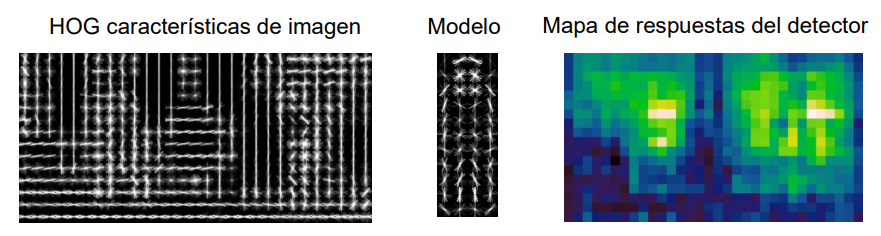
\includegraphics[width = \textwidth]{figs/deteccion-dalal.png}
\end{figure}

\begin{table}[h]
\centering
\begin{tabular}{p{6.5cm}|p{6.5cm}}
Ventajas del detector Dalal-Triggs & Desventajas del detector Dalal-Triggs \\ \hline
Funciona aceptablemente para objetos no deformables con orientaciones canónicas: caras, coches, personas & Requiere grandes cantidades de datos para entrenamiento \\
Detección rápida & No es robusto a oclusiones \\
 & Rendimiento bajo para objetos altamente deformables
\end{tabular}
\end{table}
%16/10 - Júlia Baguña Torres
\chapter{Aplicaciones en la Tomografía por Emisión de Protones}
\section{Fundamentos físicos de la imagen PET}
La imagen médica nuclear para la medicina de precisión implica el uso de trazadores (radiofármacos) para evaluar las funciones corporales y para diagnosticar enfermedades. Dentro de las imágenes médicas nucleares están PET (\textit{Positron Emission Tomography}) y SPECT (\textit{Single-Photon Emission Computed Tomography}). Estas técnicas dan información sobre la distribución de un radiofármaco, pudiendo detectar enfermedades en fases más tempranas que otras que miden el cambio anatómico estructural que suelen aparecer más tarde en la enfermedad. Como van dirigidas a dianas moleculares, tienen una alta sensibilidad, no son invasivas, a tiempo real, imágenes 3D y a nivel de todo el cuerpo, proporcionan información funcional y metabólica, se puede adquirir en distintos puntos de tiempo (adquisición longitudinal) y permite la cuantificación.

La imagen médica nuclear permite la detección de la enfermedad, estadificación, caracterización molecular, monitorización del efecto terapéutico, desarrollo y optimización de nuevos fármacos y theranostics (mira lo que tratas y trata lo que ves).

En medicina nuclear, el concepto central es el radiofármaco o trazador adminsitrado. El trazador es un agente de contraste que debe cumplir con tres principios:
El trazador se administra en cantidades traza, una concentración muy pequeña a nivel picomolar para poder visualizar un proceso fisiopatológico pero sin perturbarlo. El trazador se utiliza para medir parámetros fisiológicos de un sistema conocido, debe ser específico. Para obtener información funcional se requiere la cuantificación absoluta de su concentración. 

El trazador suele estar formado por dos entidades. El vector molecular dirige el trazador a la diana molecular, pudiendo ser una molécula pequeña, péptido, anticuerpo, fármaco, célula, etc. Por otra parte está el radionúclido, que es la señal que se detecta. La vida media de un radioisótopo es el tiempo en el que pierde la mitad de su radiación. Además, los radiofármacos pueden tener distintos tipos de emisión. Los radionúclidos que se utilizan para radioterapia dirigida suelen emitir $\alpha$ y $\beta$, mientras que los $\gamma$ se suelen utilizar para el diagnóstico. 

En SPECT, se utilizan radioisótopos que emiten radiación gamma directamente. Los detectores son cámaras gamma con estructuras de colimadores. Para ubicar el lugar de emisión, se utilizan los colimadores para filtrar las emisiones en un ángulo o localización determinada. Al hacerlo así, se pierden varios eventos en la misma detección, por lo que es menos sensible que PET. Las cámaras gamma van girando alrededor del paciente para capturar las imágenes 2D que en la reconstrucción posterior se convierte en 3D con la emisión del paciente. Como las cámaras se van moviendo y el campo de visión es relativamente pequeño, es difícil detectar radiación a tiempo real. No obstante, estos radioisótopos gamma suelen emitir radiación gamma de distintas energías, pudiendo así detectar ventanas de energías específicas (por ejemplo para varios fármacos). 

El PET está basado en la detección de positrones emitidos por el radioisótopo. El positrón viaja una corta distancia y se suele encontrar con un electrón del tejido. Se produce un evento de aniquilación que causa dos rayos gamma en sentido opuesto. Los detectores son redondos alrededor de todo el cuerpo, por lo que no es necesario que se muevan y la sensibilidad es mucho mayor.  

\section{Radiotrazadores}
Uno de los trazadores más utilizados es FDG o fluorodeoxiglucosa. Este trazador es un análogo de la glucosa, pudiendo así comportarse igual que la glucosa en los dos primeros pasos de la glucólisis. Se fosforila dentro de la célula y queda así atrapada. El trazador se utiliza al ser un análogo de la actividad glucolítica y proliferativa de la célula. Los tumores tienen una alta capacidad glucolítica, siendo así un método fiable para captar órganos que no procesan la glucosa de forma normal o enfermedades metabólicas. 

Las modalidades anatómicas de imagen miden modalidades anatómicas del tejido. En TAC, se mide la capacidad de absorción de los rayos X. En la resonancia magnética, se mide la densidad de protones y cómo afectan distintas secuencias a perfusión, difusión, etc. En PET, cada vóxel representa la concentración del trazador administrado en unidades de kilobequerelio/mL. Estas medidas se convierten posteriormente en parámetros fisiológicos relacionados con el proceso biológico o biomarcador de interés.

\section{Métodos de reconstrucción y pre-procesamiento de imagen PET}

Hay muchos factores que afectan a la calidad PET, por lo que es necesario hacer un control de calidad de los datos PET. Hay factores asociados al momento de preadquisición de la imagen, adquisición y postadquisición de la imagen.

\subsection{Pre-reconstrucción de la imagen}
Es importante tener una aproximación precisa de la dosis inyectada. La dosis inyectada se mide con un activímetro, necesitando una buena cross-calibración entre el activímetro y el detector. Es importante escoger una dosis adecuada. Si se inyecta poca cantidad, habrá una baja resolución espacial y mucho ruido de fondo, teniendo una baja reproducibilidad en la cuantificación. Si la dosis es muy alta, quizás se superan los umbrales del escáner PET y llegar a un punto de saturación de la imagen, causando artefactos. Por otro lado se debe optimizar el tiempo de escaneo para asegurar que se registren suficientes eventos. Un tiempo demasiado breve tendrá pocas cuentas y una imagen ruidosa, pero un tiempo excesivo tiene un alto coste y el paciente estará incómodo. Por ello se debe hacer una precalibración para ajustar el escáner a la escala del activímetro. Hay que tener siempre en cuenta el decaimiento del radioisótopo, el tiempo transcurrido entre la inyección y la adquisición. 

\subsection{Reconstrucción de imagen PET}
La reconstrucción es el proceso mediante el cual se convierten los datos crudos de las proyecciones adquiridas a la imagen 3D de la distribución del radiotrazador. La calidad de la imagen PET depende de:
\begin{itemize}
\item Contraste: intensidad de la imagen
\item Resolución: nivel de detalle de la imagen
\item Ruido: homogeneidad de la imagen
\end{itemize}

Los parámetros de reconstrucción afectarán a la calidad global. Hay dos tipos de métodos de reconstrucción: analíticos e iterativos. El \textbf{algoritmo analítico} se llama retroproyección filtrada, y todas las proyecciones se filtran para generar el objeto original. Este método es rápido y preciso para objetos de geometría simple y tiene pocos requisitos computacionales. No obstante, puede causar artefactos de línea o estrella, pérdida de resolución y correcciones físicas son difíciles de implementar. La \textbf{reconstrucción iterativa} suele partir de una estimación del objeto inicial, la cual se va refinando en sucesivas iteraciones en las que se compraran las proyecciones estimadas con las proyecciones reales. La resolución final es mejor y se pueden implementar las correcciones físicas, pero la reconstrucción es lenta y convergencia no uniforme, además de tener altos requisitos computacionales. 

Los métodos iterativos pueden tener un distinto número de iteraciones o subsets. Números insuficientes producen imágenes suavizadas y de bajo contraste, mientras que un valor demasiado alto tendrá una resolución espacial extrema e imágenes ruidosas.

Las correcciones físicas de la imagen PET son:
\begin{itemize}
\item \textbf{Atenuación}: absorción de los rayos gamma por parte del tejido a través del efecto fotoeléctrico o dispersadas fuera del ángulo del anillo de detección. En humanos se puede llegar a perder el 50-75\% de señal si no se aplica la corrección.
\item \textbf{Dispersión (scatter):} los rayos gamma pueden colisionar con una partícula cargada, perder parte de su energía y cambiar de dirección para cuando llega al detector. El impacto de la dispersión se corrige muy bien si se corrige la atenuación.
\item \textbf{Randoms:} detección dentro de la misma ventana de tiempo de 2 rayos gamma individuales, generando una falsa coincidencia.
\end{itemize}

En la práctica clínica habitual suele haber modelos híbridos, imágenes de PET junto con imágenes de resonancia o TAC. Este corregistro permite tener una referencia anatómica y una segmentación más precisa de órganos y tejidos.
Hay un corregistro con algoritmos de software (rígido, afín, no rígido y deformable), con marcadores fiduciales, basado en puntos anatómicos y con gating.

El PET es una imagen bastante ruidosa, teniendo que aplicar filtros después de la reconstrucción (nunca antes). Estos filtros ayudan a definir las estructuras anatómicas, aunque se deben evitar con pocos eventos.

\section{Métodos de cuantificación}
La cuantificación de la imagen PET también puede verse afectada por el método de análisis escogido: órgano a segmentar, información a obtener, si está bien delimitado el tejido. 

\subsection{Efecto de volumen parcial}
PET no se caracteriza por tener una resolución buena. Generalmente se observa un efecto de derrame en el que la actividad de los vóxeles se derrama sobre las estructuras adyacentes. Se subestima la concentración de actividad en la estructura (disminuye) y se incrementa la captación en las estructuras adyacentes. Este efecto se ve agravado cuando en un vóxel hay una mezcla de estructuras. Además, hay movimientos del paciente que afectan a la resolución de la imagen.

\subsection{Volúmenes de interés (VOIs) manualmente delinados en PET}
Para estimar la concentración de trazador en un nódulo linfático: ¿Es una buena estrategia dibujar un VOI en el nódulo y extraer la concentración de actividad media? No, porque al ser una estructura tan pequeña, habrá un efecto de volumen parcial terrible. Es difícil definir los límites anatómicos en una imagen PET. Los límites del VOI no afectan al valor de actividad máximo dentro del mismo. El valor máximo dentro de un VOI es muy sensible al ruido.
Solución: Dibujar un pequeño VOI dentro de la zona más “caliente” (radioactivo) de la región de interés.

Para ciertos tejidos, se puede estimar la concentración media del trazador siempre que la señal sea homogénea, la región sea mucho más grande que la resolución del escáner y que los límites anatómicos estén claros.

\subsection{VOIs delinados mediante thresholding}
Este método consiste en la segmentación semi-automática seleccionando vóxels por encima de un valor predeterminado o umbral ($0.25 \cdot max$, $0.5 \cdot max$, etc). Este método permite una buena estimación de la concentración media de la actividad, pero para definir el valor límite óptimo se requiere de una pre-calibración del escáner.

\subsection{VOIs delinados en imágenes anatómicas}
En sistemas híbridos, segmentación directa sobre la imagen anatómica coregistrada con el PET (CT, MRI). Estas modalidades permiten una delinación del VOI precisa y una estimación robusta de la concentración media, pero es dependiente de la resolución espacial de la modalidad anatómica, y no es aplicable a todos los tejidos.

\subsection{VOIs delineados usando plantillas anatómicas}
Se usan plantillas anatómicas (atlas) con VOIs predefinidas. Se utiliza generalmente para PET cerebral.
Permite rotación, translación y transformación no rígida, pero estas plantillas no se suelen usar para todos los órganos al ser deformable y no poder usarse en regiones blandas. En el caso del cerebro, como está protegido por el cráneo, sí se puede utilizar este método.

\subsection{Segmentación next-generation con IA}
Hay métodos con inteligencia artificial que permiten segmentar de forma más rápida y objetiva. Se extraen múltiples parámetros de cuantificación y un análisis multimodal. 

\subsection{Cuantificación}
La concentración del trazador administrado no es equivalente al proceso fisiológico relacionado. El proceso biológico está directamente relacionado con la concentración de trazador específicamente unido a células o biomarcadores moleculares (receptores, enzimas, transportadores, etc.)

Concentración específica de trazador $\neq$ concentración total de trazador

Habrá una fracción de trazador en sangre, trazador libre en el tejido, captación no específica del trazador, captación específica del trazador, metabolitos radioactivos asociados al trazador.

La señal PET es proporcional a la captación específica del trazador en trazadores altamente específicos, o cuando la concentración libre del trazador en tejido o la concentración del trazador en sangre son muy bajos. En cualquier caso, esto es información desconocida para nuevos trazadores. 

\subsection{PET dinámico y modelaje farmacocinético}
Para estudiar un trazador nuevo se realiza un estudio de PET dinámico. Se utiliza una adquisición larga y se generan imágenes con un binning temporal específico para estimar la concentración del trazador a lo largo de un periodo de tiempo.

El modelaje cinético utiliza la información de las TACs pero también de la concentración libre de trazador en sangre disponible en función del tiempo (\textbf{función input}). La concentración de trazador en sangre en función del tiempo generalmente se estima directamente de la sangre (muestreo arterial). En el proceso de imagen dinámica se le pone al paciente una cánula y de ahí se van sacando durante el escáner muestras de sangre que se separan en fracciones plasmática y analizar la muestra plasmática por cromatografía líquida de high performance. 

Hay otros métodos menos invasivos para estimar la función input:
\begin{itemize}
\item A partir de sangre venosa
\item Derivada de la imagen si es que hay un vaso sanguíneo visible en la imagen
\item Basados en estudios poblacionales, aunque no tienen en cuenta la variabilidad interindividual 
\item Basada en un tejido de referencia
\end{itemize}

\section{Modelaje farmacocinético}
Toda la información se debe combinar para obtener la concentración de trazador específica. El problema es que hay muchas constantes cinéticas, teniendo así riesgo de sobreajuste. 

\subsection{Modelo de 1 compartimento de tejido}
En este caso se considera un compartimento del tejido, que es el del trazador específicamente unido.  La aproximación es que la concentración libre e inespecífica es 0. Mediante constantes diferenciales se pueden estimar las constantes de entrada y salida. 

\subsection{Modelo de 2 compartimentos de tejido}
Es otra simplificación del modelo general. Se puede medir el potencial de unión mediante las constantes de entrada y salida. Es el patrón más utilizado, especialmente en receptores cerebrales. 

Sobre este modelo se puede asumir que el trazador no puede salir como ocurría con FDG.

\subsection{Modelos de tejido de referencia}
Se utilizan las curvas tiempo-actividad de un tejido de referencia que no expresa el biomarcador de interés. No se extraen muestras de sangre.

\section{Imagen PET dinámica vs estática}
Para obtener información cuantitativa, se debe escanear siempre de forma dinámica. Es una información necesaria de tener y en ningún caso se pueden hacer extrapolaciones de resultados de cuantificación a parámetros fisiológicos sin PET dinámico.

En algunos casos se ha logrado partir de una imagen PET estática y sacar medidas cuantitativas, como el procentaje de dosis inyectada o SUV (standardized uptake value).

\subsection{Standardised uptake value}
$$SUV = \frac{\text{Activity voxel concentration in VOI}}{\text{injected dose / patient weight}}$$

El SUV se puede equiparar con la concentración de trazador unido específicamente a su diana en el caso de trazadores altamente específicos y cuando la concentración libre del trazado en tejido y cuando la concentración del trazador en sangre son muy bajas. Esta medida no deja de ser semicuantitativa.

Se puede utilizar un SUV ratio del SUV del tejido / SUV referencia como alternativa siempre que exista una región de referencia que tenga una señal homogénea, sin captación específica del trazador y que permita la delineación de VOIs suficientemente grandes.

\section{Puntos clave}
La cuantificación de imágenes PET es el resultado de un proceso complejo que incluye la adquisición de datos, su reconstrucción, el análisis de imagen y el modelaje cinético.

Para garantizar que la estimación de la concentración del trazador es precisa:
\begin{itemize}
\item Inyectar la cantidad de actividad óptima y escoger el protocolo de escaneo adecuado
\item Aplicar el protocolo de reconstrucción óptimo y aplicar las correcciones de datos pertinentes
\item Optimizar el método de análisis de imagen para obtener la información deseada
\end{itemize}

Para garantizar que se está cuantificando la concentración de trazador específicamente unida a la diana de interés:
\begin{itemize}
\item Se deben realizar estudios dinámicos de PET y aplicar el modelo cinético adecuado
\item Se recomienda obtener la función input arterial
\item En caso de no ser posible, se puede considerar aplicar modelos de tejido de referencia o métodos estáticos
\end{itemize}

\end{document}
